% !TeX encoding = UTF-8
%% \textbf{重庆大学}通用毕业论文\LaTeXe{}模板
%%% 使用前请先阅读使用文档和用户协议,内有详细介绍。Happy Texing! :)
%% =======================================================
\documentclass%
	[type=master, bilinguallist=apart, 
	printmode=oneside, blindtrail=true]{cquthesis}%
% 可用选项:
% type=[bachelor|master|doctor],      % 必选,毕业论文类型,以下项目不填时为默认
% liberalformat,                      % 可选,仅适用本科生,使用文学类论文标题格式,默认未打开
% proffesionalmaster=[true|false],    % 可选,仅适用研究生,是(true)否(false)专业硕士,默认为否
% printmode=[oneside|twoside|auto],	  % 可选,论文打印方式,默认采用auto按页数要求自动判定
% openany,|openright,                 % 可选,双面打印时每章的第一页仅右页开启,默认右页开启(openright)
% bilinguallist=[off|combined|apart], % 可选,图录表录等分别按双语题注混编(combined),分开编录(apart),默认关(off)
% blindtrail=[true|false],                         % 可选,盲审模式,开启后封面姓名和致谢部分会隐藏,详情请参阅用户文档,默认关
% draft,                              % 写作期间可选,不渲染图片,关闭外围功能,加快预览速度,默认未开启

% 请在cquthesis.sty文件中定义其他会用到的宏包和自己的变量
% 这样可以防止main.tex太过臃肿。
\usepackage{cquthesis}

% 定义所有的图片文件在 figures 子目录下
\graphicspath{{figures/}}

% 定义数字圆
\usepackage{tikz}
\newcommand*\circled[1]{\tikz[baseline=(char.base)]{
            \node[shape=circle,draw,inner sep=1pt] (char) {\small #1};}}

%*** 写作时,使用这个命令只渲染你想查看的部分,提升工作效率,定稿时注释掉整行
% \includeonly{contents/introduction}
% \includeonly{contents/related_work}
% \includeonly{contents/MGRCL}
% \includeonly{contents/S2V}


\begin{document}


\cqusetup{
%	************	注意	************
%	* 1. \cqusetup{}中不能出现全空的行,如果需要全空行请在行首注释
%	* 2. 不需要的配置信息可以放心地坐视不理、留空、删除或注释(都不会有影响)
%	*
%	********************************
% ===================
%	论文的中英文题目
% ===================
  ctitle = {待补充},
  etitle = {待补充},
% ===================
% 作者部分的信息
% \secretize{}为盲审标记点,在打开盲审开关时内容会自动被替换为***输出,盲审开关默认关闭
% ===================
  cauthor = \secretize{尹国伟},	% 你的姓名,以下每项都以英文逗号结束
  eauthor = \secretize{Guowei~Yin},	% 姓名拼音,~代表不会断行的空格
  studentid = \secretize{},	% 仅本科生,学号
  csupervisor = \secretize{黄~~~晟~~~~~教授},	% 导师的姓名
  esupervisor = \secretize{{Prof.~Sheng Huang}},	% 导师的姓名拼音
  cassistsupervisor = \secretize{}, % 本科生可选,助理指导教师姓名,不用时请留空为{}
  cextrasupervisor = \secretize{}, % 本科生可选,校外指导教师姓名,不用时请留空为{}
  eassistsupervisor = \secretize{}, % 本科生可选,助理指导教师或/和校外指导教师姓名拼音,不用时请留空为{}
  cpsupervisor = \secretize{}, % 仅专硕,兼职导师姓名
  epsupervisor = \secretize{},	% 仅专硕,兼职导师姓名拼音
  cclass = \secretize{\rmfamily{2025}\heiti{年}\rmfamily{5}\heiti{月}},	% 博士生和学硕填学科门类,学硕填学科类型
  research_direction = \zihao{3}{工学},
  edgree = {},	% 专硕填Professional Degree,其他按实情填写
% % 提示:如果内容太长,可以用\zihao{}命令控制字号,作用范围:{}内
  cmajor = 工~~~~学,	% 专硕不需填,填写专业名称
  emajor = , % % 专硕不需填,填写专业英文名称
  cmajora = \zihao{3}{软件工程},
  cmajorb = \zihao{3}{计算机视觉},
  cmajorc = \secretize{},
  % cmajord = 2024年6月,
% ===================
% 底部的学院名称和日期
% ===================
  cdepartment = ,	%学院名称
  edepartment = ,	%学院英文名称
% ===================
% 封面的日期可以自动生成(注释掉时),也可以解除注释手动指定,例如:二〇一六年五月
% ===================
%	mycdate = {2023年6月},
%	myedate = {June 2023},
}% End of \cqusetup
% ===================
%
% 论文的摘要
%
% ===================
\begin{cabstract}	% 中文摘要
针对问题一,首先将题目中 BT.2020 和显示屏色域(sRGB)的色度坐标转换为"设备无关"的 XYZ 三刺激值,并基于此三刺激值转换为 CIELab 空间。我们选择专业的广泛使用的 $\Delta E_{2000}$ 色差公式,并以其为优化目标,使用差分进化算法对其进行优化。最后得到视频源色域到显示屏色域的 XYZ 三刺激值转换矩阵。将转换后的结果与原显示屏色域相比可以得到极低的 $\Delta E_{2000}$ 损失值以及色度图面积差值。说明此模型具有极低的感知误差以及对目标色域的高保真拟合。

针对问题二,我们通过训练一个神经网络来学习从四通道RGBV输入到五通道RGBCX输出的映射关系。为此,设计了一个 ColorNet(一个简单的多层感知器),其输入层接收4个特征(RGBV),输出层产生5个特征(RGBCX)。训练过程使用了一个合成数据集,该数据集通过受控的非线性变换生成,以模拟现实世界的复杂性。最小化颜色转换损失的关键在于自定义的 CombinedLoss 函数。该函数结合了两种损失成分:均方误差(MSE),$\Delta E_{2000}$,通过对这两种损失成分进行加权,模型在保持整体通道一致性的同时,优先考虑感知上准确的色彩再现。模型使用AdamW优化器进行训练,并通过跟踪训练损失和验证损失来评估其性能。最后,解决方案包括ΔE2000误差分布、输入和输出系统色域的色度图以及样本颜色预测的可视化,以评估学习到的映射的有效性。

针对问题三,建立了基于CIE Lab色彩空间和三基色原理的LED显示器颜色校正模型。该模型结合伽马校正与线性矩阵变换,采用差分进化算法优化校正参数,实现精确的颜色还原。首先,通过对数线性回归估计LED显示器的伽马参数,发现主色通道(如红色图像的R通道)的伽马值显著较小(约0.022),而非主色通道的伽马值相对较大(约0.23),体现了LED显示器在不同颜色通道上的非线性响应特性差异。然后,设计包含色差损失、正则化项和行列式惩罚的综合目标函数,基于CIE $\Delta E_{00}$色差公式构建优化目标。采用全局-局部混合优化策略:先用差分进化算法进行全局搜索,再用L-BFGS-B方法进行局部精调。实验结果表明,三种基色图像的平均色差从2.0以上降低到0.1左右,平均改善幅度达95.6\%;校正后100\%像素的色差均小于1.0,达到人眼难以察觉的优秀标准;校正矩阵行列式值约0.10,保证了数值稳定性和变换可逆性。该模型为LED显示器颜色处理提供了完整的理论框架和实用的工程解决方案。
\end{cabstract}
% 中文关键词,请使用英文逗号分隔:
\ckeywords{颜色空间转换;LED显示器校正;CIE Lab色彩空间;$\Delta E_{00}$色差;差分进化;神经网络;伽马校正;多通道颜色系统}

% 封面和摘要配置完成
% 封面部分
% \makecover

\frontmatter %%%前置部分(封面后绪论前)
\cquauthpage[contents/cover1.pdf]
%\cquauthpage[contents/cover2.pdf]
%\cquauthpage[contents/cover3.pdf]
%\cquauthpage[contents/cover4.pdf]

%% 原创声明和授权说明书,可选:用扫描页替换
%\cquauthpage[authscan.pdf]
%\cquauthpage

% 摘要
\makeabstract

%% 目录,注意需要多次编译才能更新
\setlength{\cftbeforetoctitleskip}{0pt}
\setlength{\cftaftertoctitleskip}{20pt}
\tableofcontents


% \setlength{\cftbeforelottitleskip}{0pt}
% \setlength{\cftafterlottitleskip}{20pt}
%% 插图索引,可选,如不用可注释掉
\renewcommand*{\listfigurename}{图目录}
\clearpage
\phantomsection
\addcontentsline{toc}{chapter}{图目录}
\listoffigures
%\listoffiguresEN
% \setlength{\cftbeforelottitleskip}{0pt}
% \setlength{\cftafterlottitleskip}{20pt}
%% 表格索引,可选
\renewcommand*{\listtablename}{表目录}
\clearpage
\phantomsection
\addcontentsline{toc}{chapter}{表目录}
\listoftables
%\listoftablesEN
%% 公式索引,可选
%\listofequations
%\listofequationsEN
%% 符号对照表,可选
% \clearpage
% \phantomsection 
% \addcontentsline{toc}{chapter}{主要符号对照表}
% % !TeX encoding = UTF-8
% 环境用两个长度参数,分别定义左边距以及词条和解释的水平距离,可自己调试以达美观(全去掉时默认:20mm,30mm)
\begin{denotation}[0mm][15mm]
	% 颜色空间相关符号
	\item[$M$] 颜色空间转换矩阵 $M\in \mathbb{R}^{3\times 3}$
	\item[$\mathbf{c}_i$] 第$i$个BT.2020 RGB颜色样本 $\mathbf{c}_i \in [0,1]^3$
	\item[$\mathbf{c}'_i$] 映射后的显示屏RGB颜色样本
	\item[$M_{BT\rightarrow XYZ}$] BT.2020色域到XYZ色彩空间的转换矩阵
	\item[$M_{DP\rightarrow XYZ}$] 显示屏色域到XYZ色彩空间的转换矩阵
	\item[$L^*$] CIE Lab色彩空间中的明度分量
	\item[$a^*$] CIE Lab色彩空间中的红绿轴分量
	\item[$b^*$] CIE Lab色彩空间中的黄蓝轴分量
	\item[$\Delta E_{00}$] CIE DE2000色差公式
	\item[$X, Y, Z$] CIE XYZ色彩空间的三刺激值
	\item[$x, y$] CIE 1931色度图坐标
	\item[$\overline{x}(\lambda), \overline{y}(\lambda), \overline{z}(\lambda)$] CIE 1931标准色度观察者匹配函数
	\item[$S(\lambda)$] 光谱功率分布函数
	
	% 神经网络相关符号
	\item[$\mathbf{X}$] 神经网络输入数据矩阵,4通道RGBV
	\item[$\mathbf{Y}$] 神经网络目标输出数据矩阵,5通道RGBCX
	\item[$W$] 神经网络权重矩阵
	\item[$\mathbf{b}$] 神经网络偏置向量
	\item[$f(\cdot)$] 激活函数
	\item[$L_{MSE}$] 均方误差损失函数
	\item[$L_{\Delta E_{2000}}$] 基于$\Delta E_{2000}$的感知误差损失函数
	\item[$L_{total}$] 混合损失函数
	\item[$\alpha, \beta$] 损失函数权重参数
	\item[$\eta$] 学习率
	
	% 差分进化算法相关符号
	\item[$\mathbf{x}_i$] 差分进化算法中第$i$个个体
	\item[$NP$] 差分进化算法种群大小
	\item[$F$] 差分进化算法变异因子
	\item[$CR$] 差分进化算法交叉概率
	\item[$\mathbf{v}_i$] 差分进化算法变异向量
	\item[$\mathbf{u}_i$] 差分进化算法试验向量
	\item[$G$] 差分进化算法迭代代数
	
	% LED颜色校正相关符号
	\item[$\gamma_c$] 第$c$个颜色通道的伽马值
	\item[$S_c$] 第$c$个颜色通道的比例因子
	\item[$I_{\text{meas},c}$] 第$c$个颜色通道的测量值
	\item[$I_{\text{target},c}$] 第$c$个颜色通道的目标值
	\item[$\mathbf{x}$] 线性RGB向量 $\mathbf{x} = [R_\ell, G_\ell, B_\ell]^T$
	\item[$\mathbf{y}$] 校正后RGB向量
	\item[$L_{\mathrm{DE}}$] 基于CIE $\Delta E_{00}$的色差损失
	\item[$L_{\mathrm{reg}}$] 正则化损失项
	\item[$L_{\det}$] 行列式惩罚项
	\item[$\mathcal{L}(M,\mathbf{b})$] LED颜色校正总目标函数
	\item[$\lambda_1, \lambda_2, \lambda_3$] 损失函数权重参数
	\item[$\epsilon$] 行列式惩罚阈值
	\item[$\text{clip}$($\cdot$, [0,1])] 数值裁剪函数,限制在[0,1]范围
	
	% 数学运算符号
	\item[$\|\cdot\|_F$] Frobenius范数
	\item[$\|\cdot\|_2$] 欧几里得范数
	\item[$\det(\cdot)$] 矩阵行列式
	\item[$I_3$] $3 \times 3$单位矩阵
	\item[$\mathbf{1}(\cdot)$] 指示函数
	\item[$\lor$] 逻辑或运算符
	
	% 其他常用符号
	\item[$N$] 样本数量
	\item[$k$] 样本索引
	\item[$c$] 颜色通道索引,$c \in \{R,G,B\}$
	\item[$\text{popsize}$] 差分进化算法种群大小
	\item[$\text{maxiter}$] 最大迭代次数
	\item[$D65$] 标准光源D65白点
	\item[$\delta$] CIE Lab转换中的阈值参数,$\delta = 6/29$
\end{denotation}

\endinput
% %% 缩略语对照表,可选
% \clearpage
% \phantomsection 
% \addcontentsline{toc}{chapter}{缩略语对照表}
% \input{contents/abbreviate}

\mainmatter %%% 主体部分(绪论开始,结论为止)
%* 子文件的多少和内容由你决定(最好以章为单位),基本原则是提速预览、脉络清晰、管理容易。

% 设置字号为小四
\renewcommand{\normalsize}{\fontsize{12pt}{20pt}\selectfont}
% 设置小四正文行间距为 20 磅
\setstretch{1.312}

\chapter[\hspace{0pt}绪论]{{\heiti\zihao{3}\hspace{0pt}绪\hskip\ccwd{}论}}\label{chapter: 绪论}
dawd\cite{MAML}
\section[\hspace{-2pt}研究背景与意义]{{\heiti\zihao{-3} \hspace{-8pt}研究背景与意义}}\label{section1: 研究背景与意义}

\section[\hspace{-2pt}问题提出与研究内容]{{\heiti\zihao{-3} \hspace{-8pt}问题提出与研究内容}}\label{section1: 问题提出与研究内容}



\chapter[\hspace{0pt}模型的假设]{{\heiti\zihao{3}\hspace{0pt}模型的假设}}

\removelofgap
\removelotgap

本章内容共分为五节,\hyperref[section2: 少样本分类]{第一节}详细介绍少样本分类任务;\hyperref[section2: 对比学习]{第二节}介绍与第三章方法相关的对比学习工作;\hyperref[section2: 语义信息表示]{第三节}介绍第四章方法应用到的语义信息表示及一些用来获得语义信息的自然语言处理模型和多模态模型;\hyperref[section2: 数据集及评价指标]{第四节}对本文所使用的数据集和评价指标进行介绍,\hyperref[section2: 本章小结]{第五节}对本章进行小结。

\section[\hspace{-2pt}少样本分类]{{\heiti\zihao{-3} \hspace{-8pt}少样本分类}}\label{section2: 少样本分类}

少样本分类,旨在模拟人类识别新类别的过程,希望模型在拥有大规模标注数据的类别上进行训练之后,能够总结并迁移所学知识到新的类别,以实现在新类别上仅用少量标注数据进行训练便能够达到良好效果的目的。与常规分类任务将数据集划分为训练集与测试集不同,少样本分类数据集被划分为基类数据和新类数据,两者类别互不相交。其中,基类数据与普通分类任务的训练集一致,所有数据均可以被用来训练模型,无论是以元学习还是以普通分类任务的训练方式。而新类数据则是用来测试模型性能,在少样本分类的测试过程中,会在新类数据集上随机采样大量分类任务,每个任务的数据又被划分为支持集与查询集,如图\ref{figure2: 少样本分类测试任务}所示。其中,支持集数据为带有标注的样本,可用来微调整个模型和重新训练分类器,而查询集作用则是类似普通分类任务中的测试集,用来评估模型准确率。根据采样任务中类别数目\emph{N}和样本数目\emph{K}的多少,其又可被称为\emph{N}-way \emph{K}-shot任务,\emph{N}通常取5,\emph{K}通常取1或5。最终,通过对大量采样任务分别进行评估,并计算这些任务的平均准确率作为模型性能的最终评价指标。

\begin{figure}[h!]
\centering
\captionsetup{font={small, stretch=1.312}}
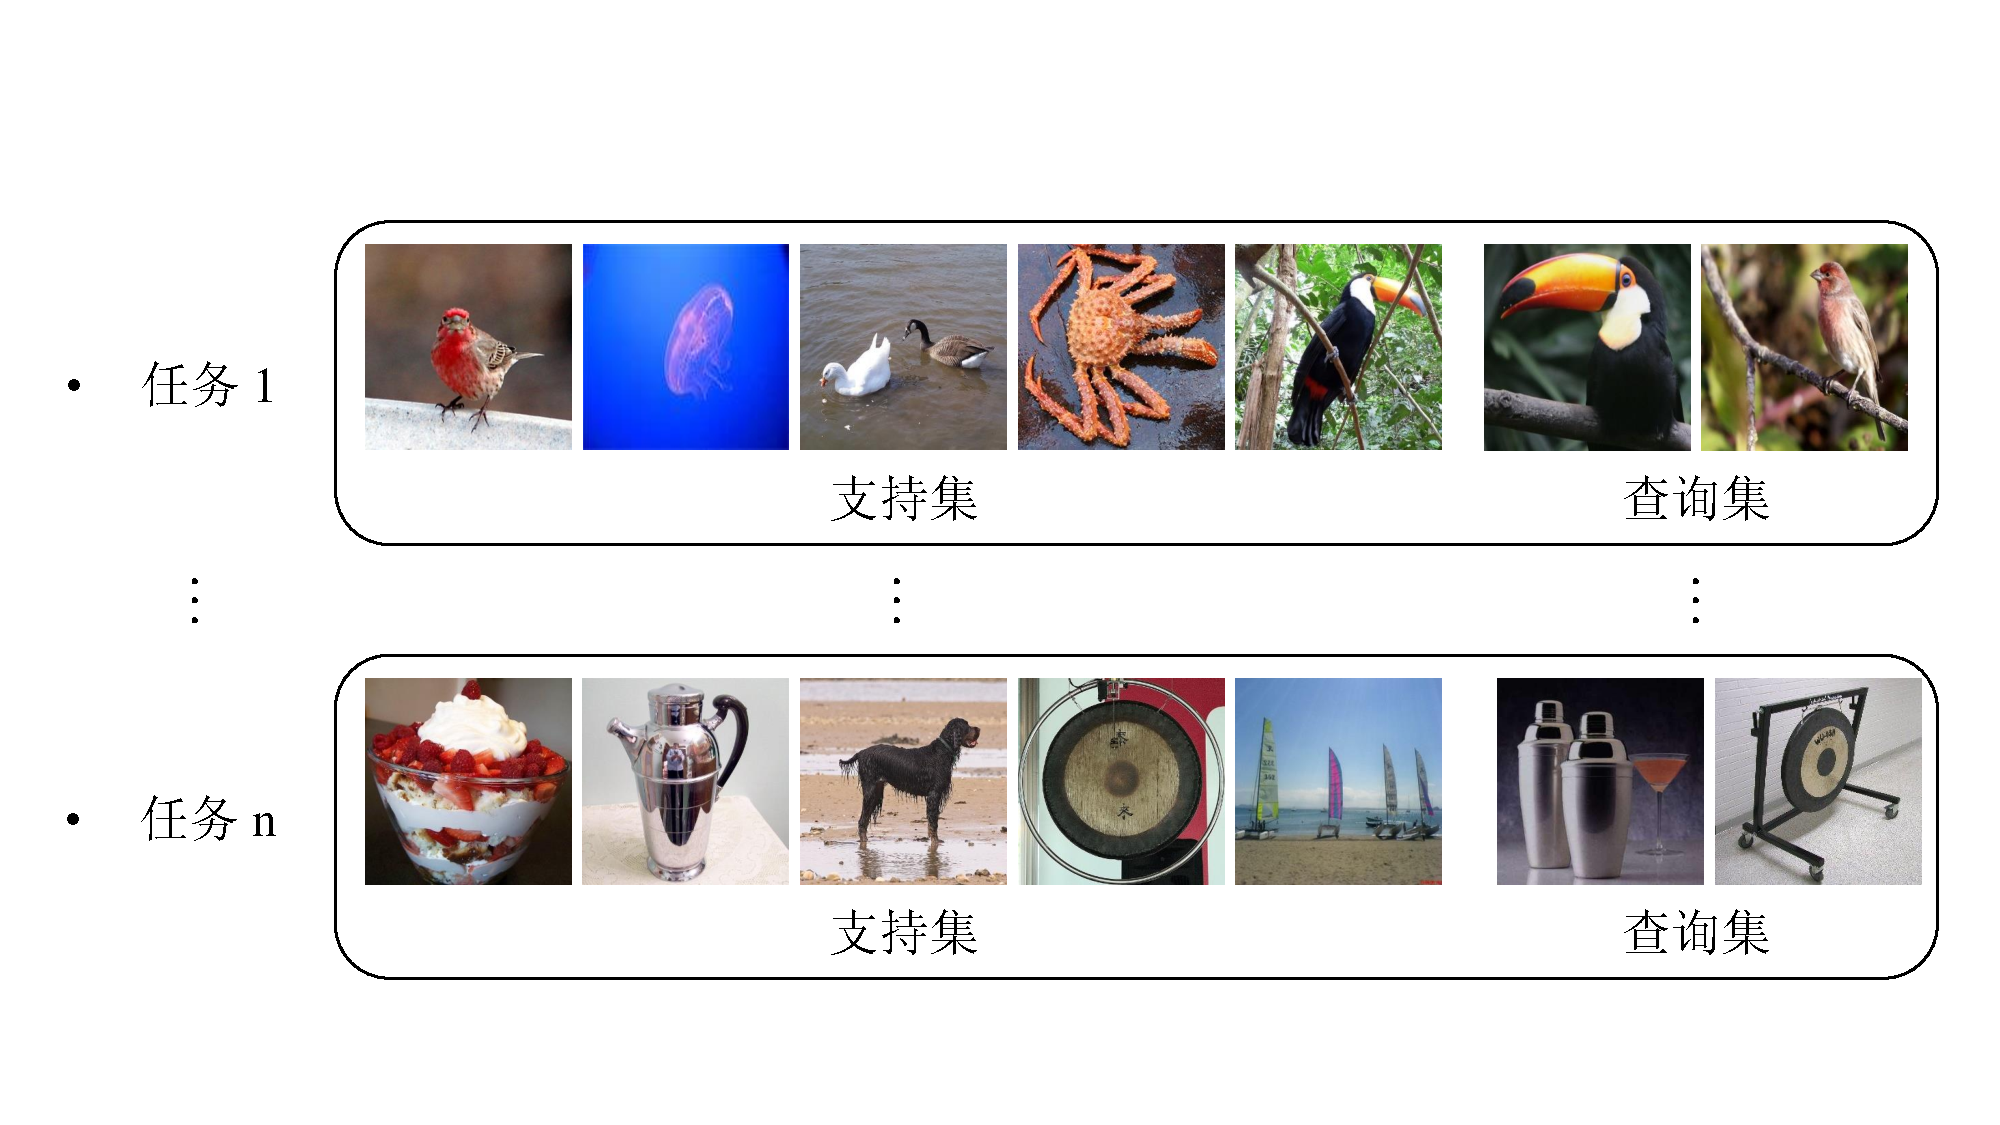
\includegraphics[width=1.0\columnwidth]{figures/RelatedWork/少样本分类测试任务.pdf}
\bicaption[少样本分类测试任务示意图]{少样本分类测试任务示意图。}[Illustration of few-shot classification testing tasks]{Illustration of few-shot classification testing tasks.}
\label{figure2: 少样本分类测试任务}
\end{figure}

\section[\hspace{-2pt}对比学习]{{\heiti\zihao{-3} \hspace{-8pt}对比学习}}\label{section2: 对比学习}

在计算机视觉领域,特征学习的方法越来越多样化。其中,对比学习以其独特的学习机制,即通过比较样本之间的相似性和差异性来提取鲜明且有区分度的特征表征,近年来受到了广泛的关注和研究。在图像处理任务中,对比学习已经证明了其在提高模型泛化能力和识别精度方面的显著效果,并被广泛应用到少样本分类问题中。根据对比学习是否使用数据集标签信息,可以将其分为无监督对比学习和有监督对比学习,以下将分别进行介绍。

\subsection[\hspace{-2pt}无监督对比学习]{{\heiti\zihao{4} \hspace{-8pt}无监督对比学习}}\label{section2: 无监督对比学习}

无监督对比学习不依赖于标注数据,它通常采用正负样本对的形式来构建训练任务。正样本对通常来自于同一实例的不同视角(例如,同一图像的不同数据增强版本),而负样本对则来自于不同实例。模型的目标是使得正样本对在表示空间中彼此接近,而负样本对彼此远离。该过程一般通过最小化InfoNCE损失函数实现,该损失函数如下式所示,
\begin{equation}
\label{equation2: infoNCE}
\mathcal{L} = - \text{log}\frac{\text{exp}(cos(f(x), f(x^+)) / \tau)}{\text{exp}(cos(f(x), f(x^+)) + \sum_{j=1}^{N} \text{exp}(cos(f(x), f(x^-))}.
\end{equation}
其中,图像$x$经由网络$f(\cdot)$后映射到特征空间,$x^+$,$x^-$分别代表$x$的正样本以及负样本,$N$为负样本数量。$cos(\cdot)$是余弦相似度,$\text{exp}(\cdot)$为以e为底的指数函数。

Chen等人\cite{SimCLR}提出了一个简单有效的无监督对比学习框架-SimCLR,旨在通过比较不同视角下图像的特征表示来学习强大的特征提取网络。SimCLR的核心思想是利用数据增强来产生正样本对,即从同一张图像中通过随机的数据增强操作(如裁剪、颜色变换等)生成两个视角,然后使来自同一图像的特征相互靠近,同时使得来自不同图像的特征尽可能地远离。尽管SimCLR在无监督特征学习方面取得了显著的成果,但其有一个明显缺点,即SimCLR的效果很大程度上依赖于对比损失函数中大量不同的负样本对,为了达到最佳性能,需要批次大小很大,这对计算资源的要求较高。He等人\cite{MoCo}提出的MoCo算法通过引入一个动态字典来存储样本特征表示解决了此问题。这个字典是一个队列,新的样本特征进入队列时,旧的样本特征被移除,以保持队列的固定大小。MoCo可通过此字典高效地采样大量负样本,因此不再需要使用很大的批次便可达到最佳效果。这些无监督对比学习方法特别适合于数据量大但未标注的场景,能够有效地利用大量未标注数据来学习有意义的特征表示。

% 通过无监督对比学习,模型能够捕捉到数据的内在结构和丰富的特征信息,这为后续的监督学习任务,如分类、检测等,提供了强大的预训练模型。此外,该方法也在自然语言处理、图数据分析等领域展现出了广泛的应用潜力。

\subsection[\hspace{-2pt}有监督对比学习]{{\heiti\zihao{4} \hspace{-8pt}有监督对比学习}}\label{section2: 有监督对比学习}

虽然无监督对比学习为使用大量无标注数据训练一个好的预训练模型提供了有效途径,但因为其在样本建模过程中将样本$x$与其负样本距离推远,而负样本中可能包含$x$的同类样本,这可能会学习到错误的样本关系。因此,Khosla等人\cite{SupCon}提出了有监督对比学习(Supervised Contrastive Learning,简称SupCon)对这个问题进行解决。SupCon是对比学习的一种变体,它结合了监督信号来进一步提升学习效率和特征表示的质量。与无监督对比学习相比,有监督对比学习在构造正负样本对时利用了标签信息,以确保模型不仅学会区分不同的样本,而且能够区分不同的类别,如图\ref{figure2: 对比学习}所示(此图来源于SupCon\cite{SupCon})。SupCon不仅保留了无监督对比学习中正样本对的概念,更进一步地,将属于同一类别的不同样本也视为正样本对,负样本对则是来自不同类别的样本,以此强化模型对不同类别间差异的识别能力。这种方法有效地缩小了同类样本间的表征距离,同时增强了不同类别间表征的区分度,有助于提升模型在复杂视觉任务中的表现。

\begin{figure}[h!]
\centering
\captionsetup{font={small, stretch=1.312}}
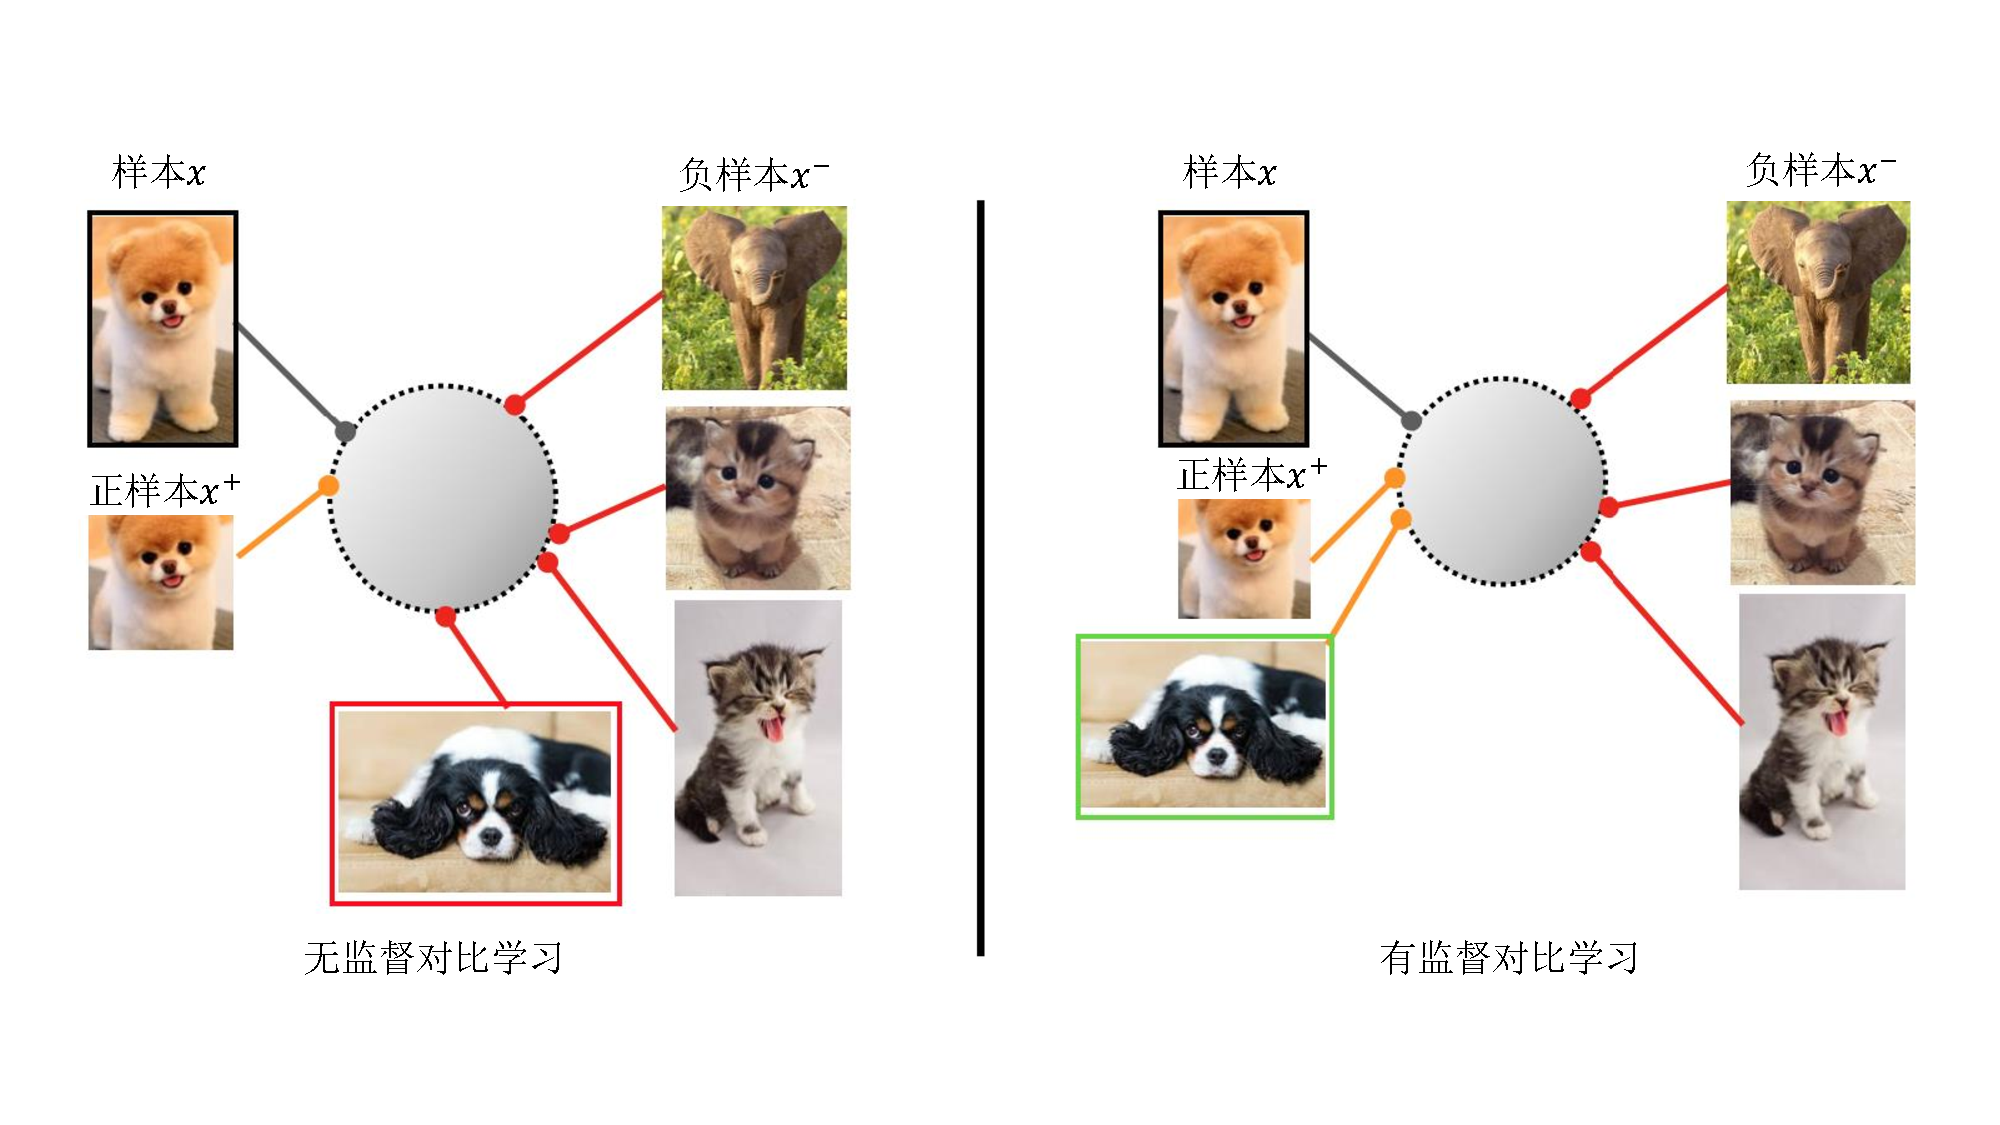
\includegraphics[width=1.0\columnwidth]{figures/RelatedWork/对比学习.pdf}
\bicaption[无监督对比学习与有监督对比学习]{无监督对比学习与有监督对比学习。}[Unsupervised Contrastive Learning VS Supervised Contrastive Learning]{Unsupervised Contrastive Learning VS Supervised Contrastive Learning.}
\label{figure2: 对比学习}
\end{figure}

\section[\hspace{-2pt}语义信息表示]{{\heiti\zihao{-3} \hspace{-8pt}语义信息表示}}\label{section2: 语义信息表示}

目前,在少样本分类问题中,很多工作开始使用语义信息以对视觉信息进行补充,使用的语义信息一般为用自然语言处理(Natural Language Processing,简称NLP)模型或多模态模型的文本编码器提取的语义特征。提取语义特征时,会将类别名称或提示文本与类别名称进行拼接之后的文本输入文本编码器,然后得到编码器输出的语义向量作为语义特征。以下对少样本分类中经常使用的语义特征提取模型进行介绍。

\subsection[\hspace{-2pt}Word2Vec]{{\heiti\zihao{4} \hspace{-8pt}Word2Vec}}\label{section2: Word2Vec}

Mikolov等人\cite{mikolov2013efficient, Word2Vec}提出的Word2Vec是一种广泛使用的自然语言处理技术,它从大量文本语料中以无监督的方式学习语义知识,旨在将词汇映射到稠密向量空间中,其中语义相似的词汇会在向量空间中彼此接近。Word2Vec包含两种训练模型:连续词袋(Continuous Bag-of-Words,简称CBOW)模型和跳跃(Continuous Skip-gram,简称Skip-Gram)模型,如图\ref{figure2: Word2Vec}所示(此图来源于Word2Vec\cite{Word2Vec})。

\textbf{CBOW模型:}CBOW模型通过上下文(周围的词汇)来预测当前词,如图\ref{figure2: Word2Vec}(左)所示。具体来说,它将上下文中的多个词汇作为输入,并尝试预测在这些上下文词汇中间的目标词汇。这个模型特别适合处理较小的数据集。

\textbf{Skip-Gram模型:}与CBOW相反,Skip-Gram模型使用一个词来预测其周围的上下文,如图\ref{figure2: Word2Vec}(右)所示。给定一个特定的词,目标是预测在一个特定范围内的前后词汇。Skip-Gram模型在处理大数据集时表现更好,尤其是对罕见词汇的表示更为有效。

\begin{figure}[h!]
\centering
\captionsetup{font={small, stretch=1.312}}
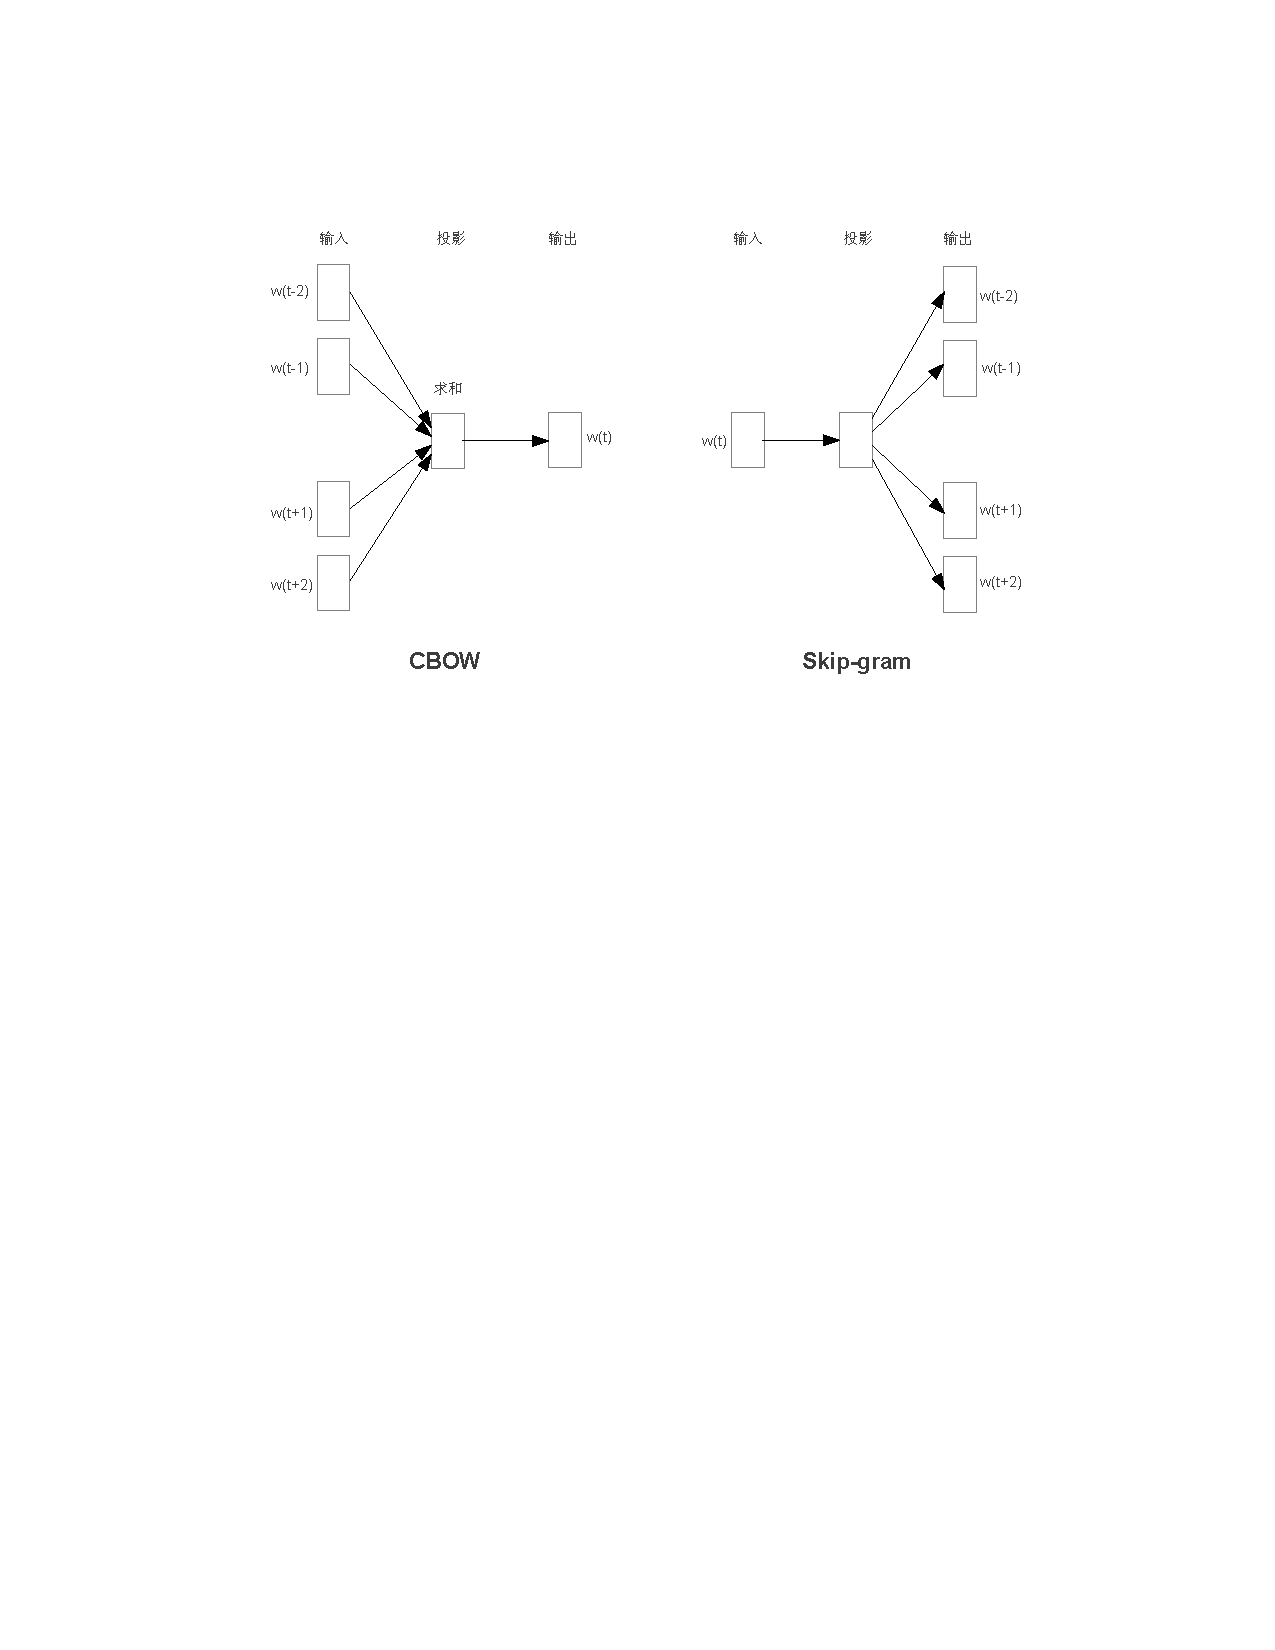
\includegraphics[width=1.0\columnwidth]{figures/RelatedWork/Word2Vec.pdf}
\bicaption[CBOW模型与Skip-Gram模型示意图]{CBOW模型与Skip-Gram模型示意图。}[Illustration of CBOW model and Skip-Gram model]{Illustration of CBOW model and Skip-Gram model.}
\label{figure2: Word2Vec}
\end{figure}

Word2Vec的核心优势在于它能够捕捉到词汇之间的细微语义关系,并通过向量运算来揭示词汇之间的语义相似性。这使得Word2Vec在诸多自然语言处理任务中得到广泛应用,包括文本相似性度量、情感分析、机器翻译以及作为深度学习模型的预训练层等,另外,很多计算机视觉任务也使用Word2Vec来提取语义特征以对视觉特征进行修正或补充。

\subsection[\hspace{-2pt}GloVe]{{\heiti\zihao{4} \hspace{-8pt}GloVe}}\label{section2: GloVe}

Pennington等人\cite{GloVe}提出的GloVe(Global Vectors for Word Representation)也是一种用于词嵌入的无监督学习算法。该模型旨在将单词映射到一个向量空间中,使得这些向量能够捕捉到词与词之间的共现关系,从而反映出词义的复杂模式和结构。GloVe模型的关键创新在于它结合了两种主流的词表示方法的优点:基于全局矩阵分解(Global Matrix Factorization)的方法和基于局部上下文窗口(Local Context Window)的方法。

GloVe的核心思想是首先构建一个全局词共现矩阵,记录整个语料库中各个词之间的共现次数,然后通过优化一个目标函数来学习词向量。这个目标函数旨在让共现次数的对数值与相应词向量的点积尽可能接近,同时引入偏置项来进一步提升模型的灵活性和准确性。具体来说,GloVe构建一个大型的词-词共现矩阵,矩阵中的每个元素代表了两个词在一定窗口大小内共同出现的次数。这一步捕获了全局的共现统计信息。然后其定义了一个特殊的损失函数,该损失函数不仅关注词对之间的共现概率,而且关注共现概率的比例,这有助于捕获词义之间更细微的差别。这个损失函数同时考虑到了共现次数的稀疏性和不均匀性。通过最小化损失函数,模型学习到的词向量能够反映出词与词之间的共现概率,这意味着词向量空间中的距离可以表示词义之间的相似度。这一步既利用了局部信息(通过具体的共现频率),也综合了全局信息(通过整个语料库的统计数据)。

\begin{figure}[h!]
\centering
\captionsetup{font={small, stretch=1.312}}
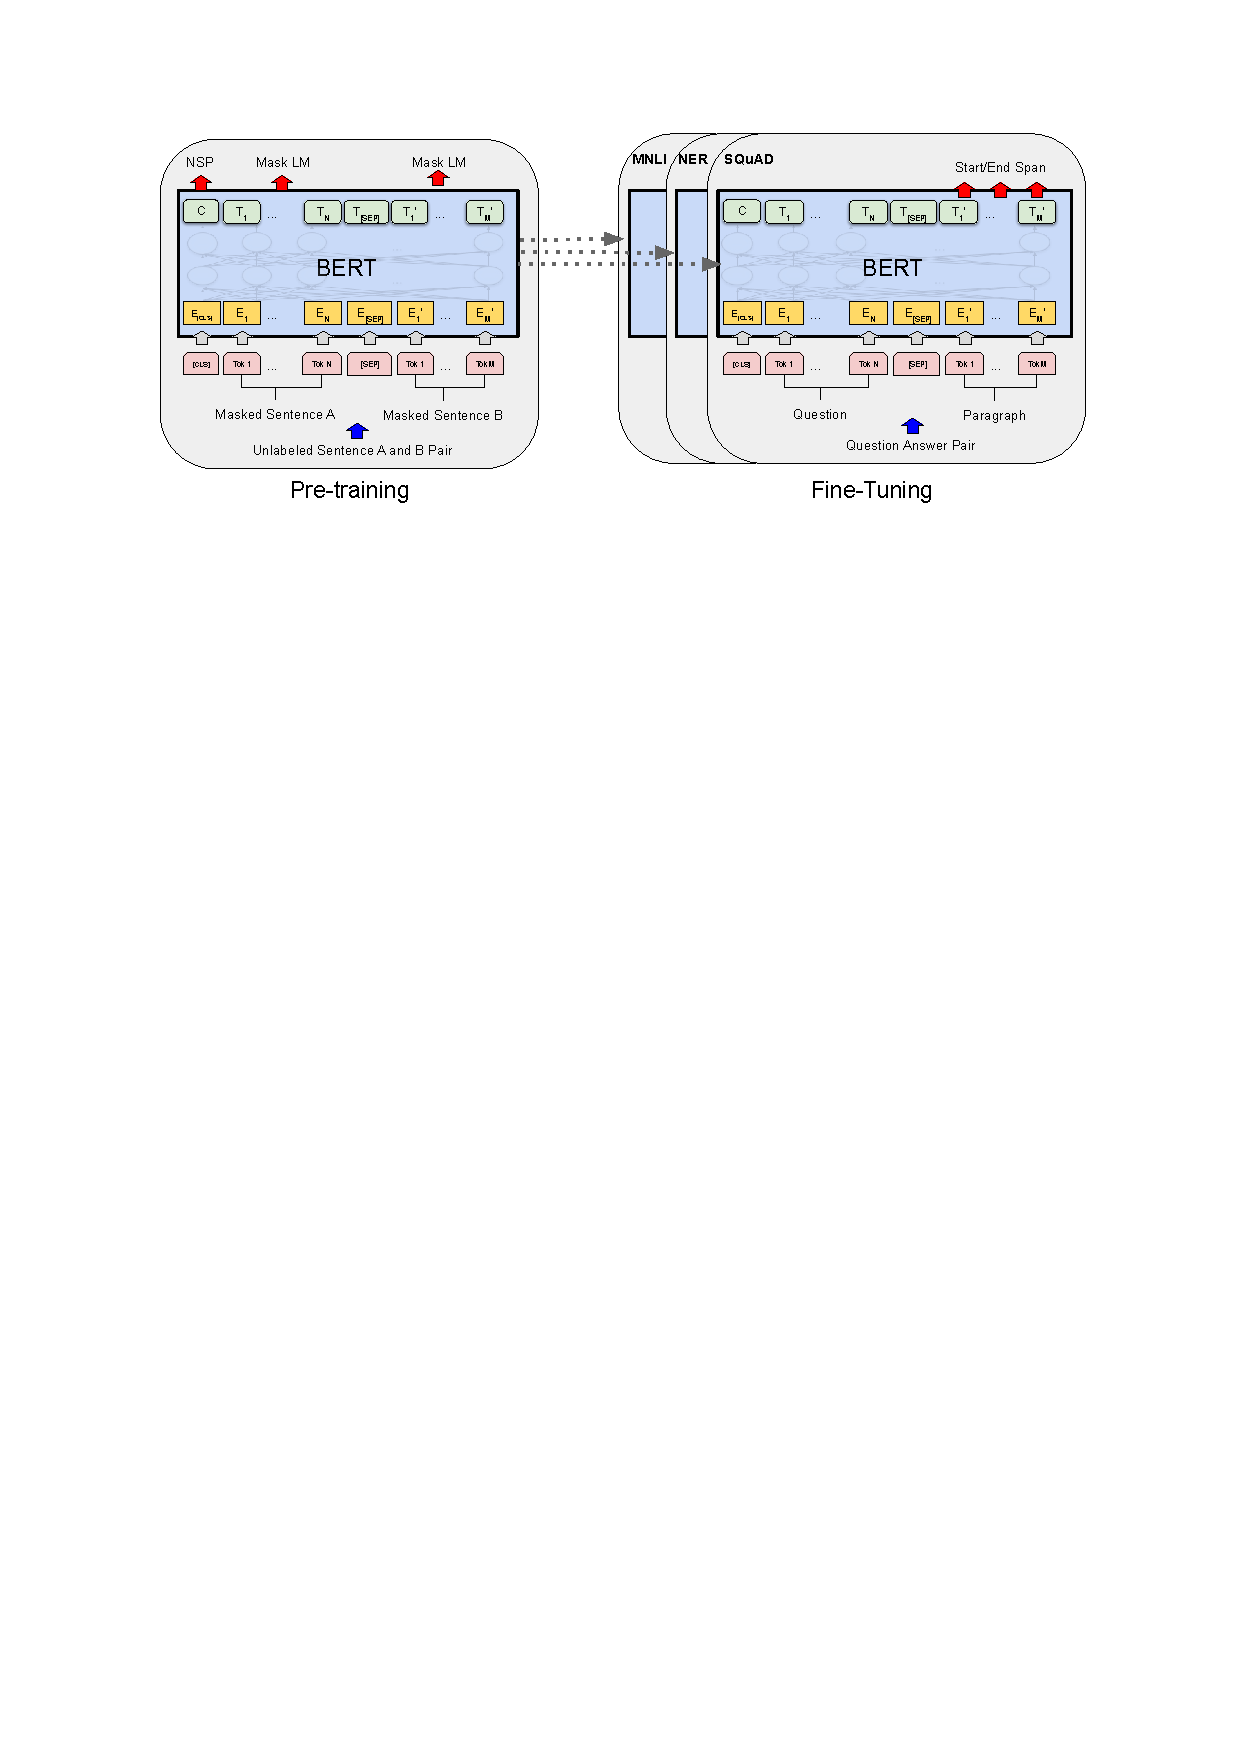
\includegraphics[width=1.0\columnwidth]{figures/RelatedWork/BERT.pdf}
\bicaption[BERT的整体预训练和微调过程]{BERT的整体预训练和微调过程。}[Overall pre-training and fine-tuning procedures for BERT]{Overall pre-training and fine-tuning procedures for BERT.}
\label{figure2: BERT}
\end{figure}

\subsection[\hspace{-2pt}BERT]{{\heiti\zihao{4} \hspace{-8pt}BERT}}\label{section2: BERT}

Devlin等人\cite{Bert}提出的BERT(Bidirectional Encoder Representations from Transformers)模型是一种革命性的自然语言处理模型。该模型利用了Transformer架构的双向编码器,能够理解语言的深层语义和上下文关系。BERT的创新之处在于其基于Transformer模型的编码器,使得它能够同时考虑词语左侧和右侧的上下文信息,这与以往的单向模型或浅层双向模型不同,使其能够更准确地理解词义。如图\ref{figure2: BERT}所示(此图来源于BERT\cite{Bert}),BERT模型首先在大规模的文本语料库上进行预训练,学习通用的语义表示,然后针对具体的NLP任务进行微调,这一过程极大提升了模型在特定任务上的性能。由于其良好的性能与开创性,后续又出现了诸如SBERT\cite{SBERT}、RoBERTa\cite{RoBERTa}、ALBERT\cite{ALBERT}等改进工作。BERT模型通过两种类型的预训练任务学习语义表示:

\noindent \textbf{(1)掩码语言模型(Masked Language Model,简称MLM):}在训练过程中,BERT会随机遮蔽模型输入句子中的一部分词语(使用[MASK] token代替原有输入),然后让模型预测这些遮蔽的词语,这可以迫使模型学习到词语的双向上下文关系。另外,为了解决模型微调期间从未看到[MASK] token的问题,BERT模型不总是直接用[MASK] token代替所选单词,而是将所选单词80\%的概率替换为[MASK] token,10\%的概率用一个随即单词替换所选单词,剩下10\%的概率则是保持其不变。

\noindent \textbf{(2)下一句预测(Next Sentence Prediction,简称NSP):}由于很多NLP下游任务都是基于理解两个句子之间的关系,如问答和自然语言推断,因此BERT设计了一个下一句预测的任务。给定两个句子A和B,模型需要预测B是否是A的下一句,这可以帮助模型理解句子间的关系。

\begin{figure}[h!]
\centering
\captionsetup{font={small, stretch=1.312}}
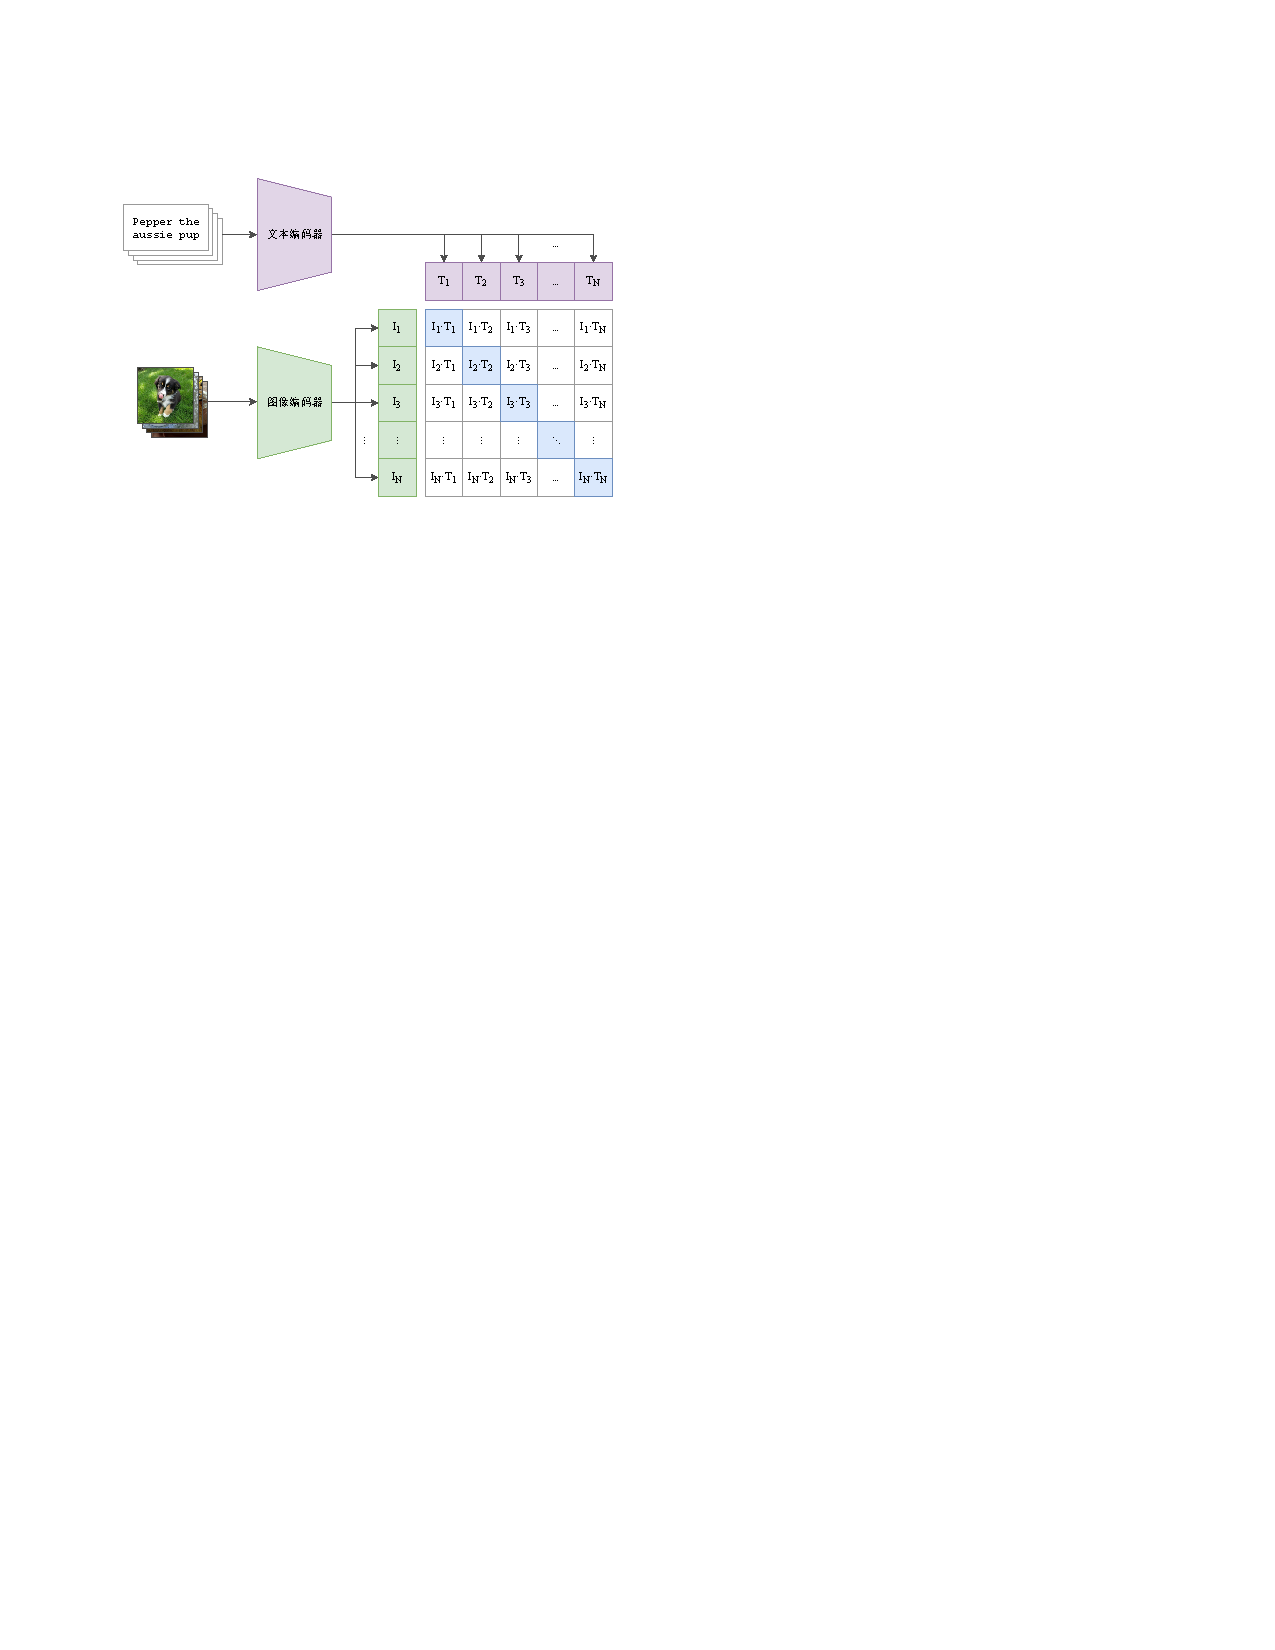
\includegraphics[width=0.8\columnwidth]{figures/RelatedWork/CLIP.pdf}
\bicaption[CLIP模型预训练示意图]{CLIP模型预训练示意图。}[Illustration of pre-training CLIP model]{Illustration of pre-training CLIP model.}
\label{figure2: CLIP}
\end{figure}

\subsection[\hspace{-2pt}CLIP]{{\heiti\zihao{4} \hspace{-8pt}CLIP}}\label{section2: CLIP}

近年来,Radford等人\cite{Clip}提出的CLIP(Contrastive Language–Image Pre-training)模型受到了很多研究者的关注,并促进了多模态大模型和一些其他任务的发展。CLIP旨在通过大规模的图文对比学习来同时理解图像和文本,并建立它们之间的联系。CLIP模型的创新之处在于其跨模态能力,它不仅能理解图片内容,也能理解与图片内容相对应的文本描述,从而在多种视觉任务上展示出了卓越的性能和强大的泛化能力,并提供了一个充分建模文本关系的文本编码器。

如图\ref{figure2: CLIP}所示(此图来源于CLIP\cite{Clip}),CLIP由两部分组成:一个图像编码器和一个文本编码器。图像编码器负责提取图像的视觉特征,而文本编码器则提取文本的语义特征。这两个编码器可以是任何形式的神经网络。在原始CLIP模型中,图像编码器基于Vision Transformer(ViT)或ResNet架构,而文本编码器基于Transformer架构。CLIP的训练过程涉及大量图像和文本对的对比学习。具体来说,模型训练的目标是最大化相匹配的图像和文本对之间的相似度,同时最小化不匹配对的相似度。这种训练方式使得CLIP学习到的特征表示能够跨越视觉和语义的界限,理解两种模态之间的对应关系。

\section[\hspace{-2pt}数据集及评价指标]{{\heiti\zihao{-3} \hspace{-8pt}数据集及评价指标}}\label{section2: 数据集及评价指标}

本文使用四个少样本分类基准数据集对模型性能进行评估,包括三个普通少样本分类数据集:miniImageNet \cite{vinyals2016matching}、tieredImageNet \cite{ren2018meta}、CIFAR-FS \cite{bertinetto2019meta},以及一个细粒度数据集:CUB-200-2011(CUB)\cite{wah2011caltech},以下对其进行分别介绍,并对少样本分类评价指标进行描述。

\begin{table}[h!]
\small    % 设置表格字体为5号
\setstretch{1.245}        % 设置具有指定弹力的橡皮长度(原行宽的1.2倍)
\captionsetup{font={small, stretch=1.512}}
\centering
\bicaption[miniImageNet、CIFAR-FS和CUB的数据集划分]{miniImageNet、CIFAR-FS和CUB的数据集划分。}[Dataset partition of miniImageNet, CIFAR-FS and CUB]{Dataset partition of miniImageNet, CIFAR-FS and CUB.}    % 中英文标题
\begin{tabularx}{\textwidth}{lCCCC}
\toprule
\multirow{2}*{数据集} & \multicolumn{4}{c}{类别数目} \\
\cline{2-5}
& \raisebox{-2pt}{训练集} & \raisebox{-2pt}{验证集} & \raisebox{-2pt}{测试集} & \raisebox{-2pt}{总数} \\
\midrule
miniImageNet & 64 & 16 & 20 & 100 \\
CIFAR-FS & 64 & 16 & 20 & 100 \\
CUB & 100 & 50 & 50 & 200 \\
\bottomrule
\end{tabularx}
\vspace{-20pt}
\label{table2: dataset1}
\end{table}

\begin{table}[h!]
\small    % 设置表格字体为5号
\setstretch{1.245}        % 设置具有指定弹力的橡皮长度(原行宽的1.2倍)
\captionsetup{font={small, stretch=1.512}}
\centering
\bicaption[tieredImageNet的数据集划分]{tieredImageNet的数据集划分。}[Dataset partition of tieredImageNet]{Dataset partition of tieredImageNet.}    % 中英文标题
\begin{tabularx}{\textwidth}{XCCCC}
\toprule
\multirow{2}*{类别层级} & \multicolumn{4}{c}{类别数目} \\
\cline{2-5}
& \raisebox{-2pt}{训练集} & \raisebox{-2pt}{验证集} & \raisebox{-2pt}{测试集} & \raisebox{-2pt}{总数} \\
\midrule
超类 & 20 & 6 & 8 & 34 \\
子类 & 351 & 97 & 160 & 608 \\
\bottomrule
\end{tabularx}
\label{table2: dataset2}
\end{table}

\subsection[\hspace{-2pt}数据集]{{\heiti\zihao{4} \hspace{-8pt}数据集}}\label{section2: 数据集}

miniImageNet数据集\cite{vinyals2016matching}和tieredImageNet数据集\cite{ren2018meta}均为ImageNet\cite{deng2009imagenet}的子集。其中,miniImageNet数据集包含100个类别,每个类别有600张图像。本文遵循Ravi等人\cite{optimization}提出的划分准则,训练集、验证集和测试集分别包含64、16和20个类别。tieredImageNet数据集则包含34个超类(608个子类),分为20个训练类别(351个子类)、6个验证类别(97个子类)和8个测试类别(160个子类)。CIFAR-FS数据集\cite{bertinetto2019meta}源自CIFAR-100数据集,该数据集包含64个训练类别、16个验证类别和20个测试类别,每个类别同样有600张图像。Caltech-UCSD Birds(CUB)-200-2011(简称CUB)数据集\cite{wah2011caltech}则是一个包含不同种类的鸟类细粒度图像数据集,包含11788个图像样本,分为200个类别。根据Triantafillou等人\cite{triantafillou2017few}的划分准则,该数据集包含100个训练类别、50个验证类别和50个测试类别。各数据集划分如表\ref{table2: dataset1}和\ref{table2: dataset2}所示。

\subsection[\hspace{-2pt}评价指标]{{\heiti\zihao{4} \hspace{-8pt}评价指标}}\label{section2: 评价指标}

对于所有数据集,本文评估5-way 1-shot 以及5-way 5-shot少样本分类任务性能。在一次模型评估中,本文方法采样2000个少样本分类任务,并计算了95\%置信区间的平均分类准确率作为模型的评价指标。在一个少样本分类任务中,每个类别的支持集样本数目为1或5(根据任务决定),查询集样本数目为15,与其他方法\cite{RFS, IER}保持一致。

\section[\hspace{-2pt}本章小结]{{\heiti\zihao{-3} \hspace{-8pt}本章小结}}\label{section2: 本章小结}

本章首先详细介绍了少样本分类任务的定义及其训练测试过程。然后对后续研究工作所涉及到的相关技术进行了介绍,其中包括第三章所使用到的对比学习技术,根据是否使用数据集标签信息将其分为无监督对比学习和有监督对比学习进行了详细阐述;以及第四章所使用到的语义信息表示,介绍了如何提取语义信息表示和少样本分类中常用的语义特征提取模型。最后,介绍了本文方法所使用到的少样本分类数据集和评价指标。

\chapter[\hspace{0pt}基于多粒度样本关系建模的少样本分类研究]{{\heiti\zihao{3}\hspace{0pt}基于多粒度样本关系建模的少样本分类研究}}\label{chapter3: 基于多粒度样本关系建模的少样本分类研究}
\removelofgap
\removelotgap
本章研究基于多粒度样本关系建模的少样本特征学习算法,通过挖掘多种粒度的样本关系并对其进行建模从而增强模型的特征提取能力,进而提升少样本分类任务的准确率。本章内容共分为四节,\hyperref[section3: 引言]{第一节}介绍研究动机和方法概述;\hyperref[section3: 基于多粒度样本关系对比学习的少样本特征学习算法]{第二节}介绍本章提出的基于多粒度样本关系对比学习的少样本特征学习算法;\hyperref[section3: 实验设置及结果分析]{第三节}给出实验设置和结果分析;\hyperref[section3: 本章小结]{第四节}对本章进行小结。

\section[\hspace{-2pt}引言]{{\heiti\zihao{-3} \hspace{-8pt}引言}}\label{section3: 引言}

\subsection[\hspace{-2pt}研究动机]{{\heiti\zihao{4} \hspace{-8pt}研究动机}}\label{section3: 研究动机}

\begin{figure}[h!]
\centering
\captionsetup{font={small, stretch=1.312}}
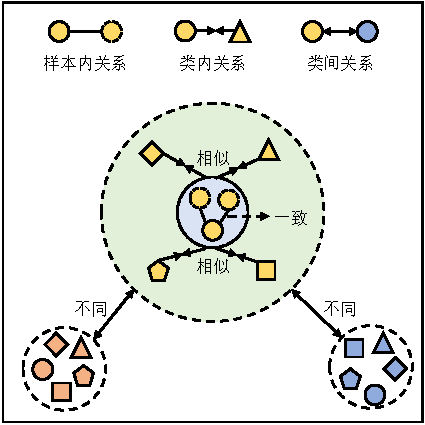
\includegraphics[width=0.6\columnwidth]{figures/MGSRCL/SampleRelation.pdf}
% \captionsetup{justification=justified,singlelinecheck=false}
\bicaption[样本关系示意图]{样本关系示意图。在该图中,不同形状与颜色分别代表不同样本与类别。同一样本的不同变换由相同的颜色和形状表示。样本关系包括三种类型:样本内关系、类内关系和类间关系。本章所提方法约束同一样本不同变换版本在语义内容上保持一致,同类样本保持相似,非同类样本保持不同。}[Illustration of sample relations]{Illustration of sample relations. In this figure, different shapes and different colors represent different samples and different classes, respectively. Different transformations of the same sample are represented by the same color and shape. The sample relations contain three types: intra-sample relation, intra-class relation and inter-class relation. The approach proposed in this chapter enforces different transformations to be consistent in semantic content, homogenous samples to be similar, and inhomogeneous samples to be different.}
\label{figure3: sample relation}
\end{figure}

\subsection[\hspace{-2pt}方法概述]{{\heiti\zihao{4} \hspace{-8pt}方法概述}}\label{section3: 方法概述}



\section[\hspace{-2pt}基于多粒度样本关系对比学习的少样本特征学习算法]{{\heiti\zihao{-3} \hspace{-8pt}基于多粒度样本关系对比学习的少样本特征学习算法}}\label{section3: 基于多粒度样本关系对比学习的少样本特征学习算法}

在本节中,首先对少样本分类任务及其符号定义进行介绍;然后对所提出的基于多粒度样本关系对比学习的少样本特征学习模型进行简要介绍;接下来详细介绍了所提模型的各个模块及其损失优化;最后介绍了模型总体优化目标以及模型推理过程。

\subsection[\hspace{-2pt}符号定义]{{\heiti\zihao{4} \hspace{-8pt}符号定义}}\label{section3: 符号定义}

在本章中,少样本分类任务的基类数据集和新类数据集分别表示为:
\begin{equation}
\begin{aligned}
  &\mathcal{D}_{base} = \{(x, y)|x \in X^{base}, y \in Y^{base}\}, \\
  &\mathcal{D}_{novel} = \{(x, y)|x \in X^{novel}, y \in Y^{novel}\}.
\end{aligned}
\end{equation}
其中,$\mathcal{D}_{base}$所包含的类别$\mathcal{C}_{base}$和$\mathcal{D}_{novel}$所包含的类别$\mathcal{C}_{novel}$不相交。另外,$x$、$y$分别表示样本图像和样本标签;$X^{base}$、$Y^{base}$和$X^{novel}$、$Y^{novel}$分别表示基类数据和新类数据的样本图像集合和标签集合。

$\mathcal{D}_{base}$用于在预训练阶段训练一个具有良好泛化性能的模型,$\mathcal{D}_{novel}$用于测试过程采样大量\emph{N}-way \emph{K}-shot少样本分类任务并计算平均准确率来评估模型性能。每个少样本分类任务$\mathcal{T}$包括一个支持集$\mathcal{S}_\mathcal{T}$和一个查询集$\mathcal{Q}_\mathcal{T}$,
\begin{equation}
  \mathcal{T} = \{\mathcal{S}_\mathcal{T}, \mathcal{Q}_\mathcal{T}\}.
\end{equation}
其中,$\mathcal{S}_\mathcal{T}$包含来自\emph{N}个类别的\emph{N} $\times$ \emph{K}个标注样本,而$\mathcal{Q}_\mathcal{T}$包含来自相同\emph{N}个类别的\emph{N} $\times$ \emph{Q}个样本,并且$\mathcal{S}_\mathcal{T}$和$\mathcal{Q}_\mathcal{T}$中的样本是没有交集的。在测试阶段,针对每个采样的少样本分类任务使用$\mathcal{S}_\mathcal{T}$重新训练一个分类器,使用$\mathcal{Q}_\mathcal{T}$来评估分类器性能。

\begin{figure}[h!]
\centering
\captionsetup{font={small, stretch=1.312}}
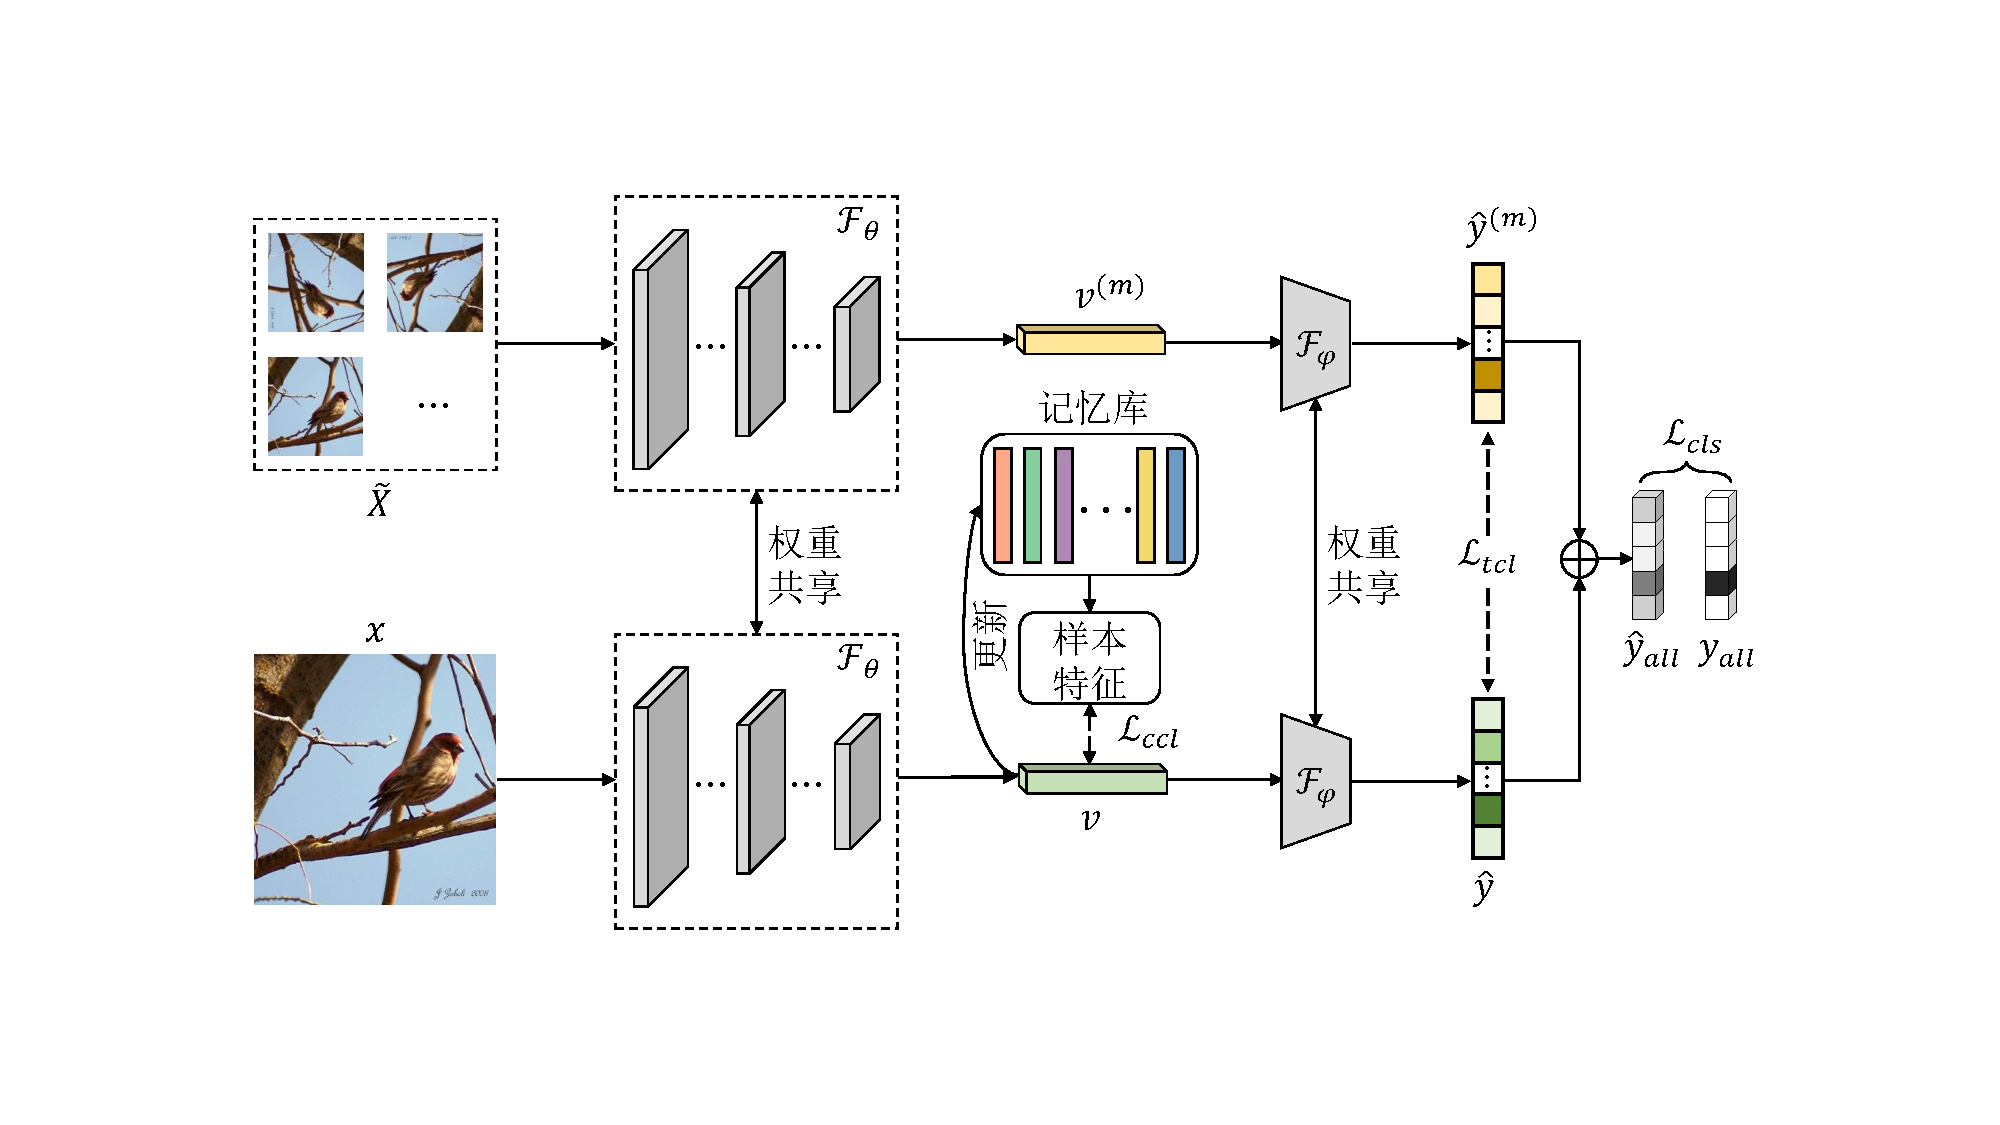
\includegraphics[width=1.0\columnwidth]{figures/MGSRCL/model.pdf}
% \captionsetup{justification=justified,singlelinecheck=false}
\bicaption[多粒度样本关系对比学习模型示意图]{多粒度样本关系对比学习模型(MGSRCL)示意图。它包含一个特征提取网络$\mathcal{F}_{\theta}$和一个分类器$\mathcal{F}_{\varphi}$。在此图中,$v$和$v^{(m)}$代表原始图像$x$及其第$m$个变换版本$x^{(m)}$的特征,其中$x^{(m)} \in \widehat{X}$。$\bigoplus$是一个连接操作,用于对原始图像的预测输出$\widehat{y}$与$M$个变换的预测输出${\widehat{y}^{(1)}, ..., \widehat{y}^{(m)}, ..., \widehat{y}^{(M)}}$进行连接。记忆库(Memory Bank)用于存储特征。$\mathcal{L}_{cls}$,$\mathcal{L}_{tcl}$和$\mathcal{L}_{ccl}$分别是分类损失、变换一致性学习(TCL)损失和类对比学习(CCL)损失。为了便于阅读,此图中没有展示自监督模块。}[Illustration of Multi-Grained Sample Relation Contrastive Learning (MGSRCL) model]{Illustration of Multi-Grained Sample Relation Contrastive Learning (MGSRCL) model. It contains a feature extraction network $\mathcal{F}_{\theta}$ and a classifier $\mathcal{F}_{\varphi}$. In this figure, $v$ and $v^{(m)}$ represent the features of the original image $x$ and its $m$-th transformed version $x^{(m)}$,where $x^{(m)} \in \widehat{X}$. $\bigoplus$ is a concatenation operator for the predicted output $\widehat{y}$ of the original image and the predicted outputs $\{\widehat{y}^{(1)}, ..., \widehat{y}^{(m)}, ..., \widehat{y}^{(M)}$\} of $M$ transformations. Memory bank is used to store the features. $\mathcal{L}_{cls}$, $\mathcal{L}_{tcl}$, and $\mathcal{L}_{ccl}$ are the classification loss, transformation consistency learning (TCL) loss, and class contrastive learning (CCL) loss, respectively. For the sake of legibility, the self-supervised module is not shown in this image.}
\label{figure3: model}
\end{figure}

\subsection[\hspace{-2pt}整体框架]{{\heiti\zihao{4} \hspace{-8pt}整体框架}}\label{section3: 整体框架}

本章重新审视了对比学习中的样本关系,并根据样本关系粒度的不同将其划分为三种类型:同一样本在不同变换下的样本内关系(intra-sample relation)、同类样本的类内关系(intra-class relation),以及不同类样本的类间关系(inter-class relation)。基于此,本章提出了一种新颖的多粒度样本关系对比学习方法(Multi-Grained Sample Relation Contrastive Learning,简称MGSRCL),通过对少样本分类中不同粒度的样本关系进行建模从而获得了一个强大的特征提取网络。如图\ref{figure3: model}所示,MGSRCL模型包含三个主要部分:基础特征学习网络(Base Feature Learning Network,简称Base)、变换一致性学习(Transformation Consistency Learning,简称TCL)模块和类对比学习(Class Contrastive Learning,简称CCL)模块。具体而言,基础特征学习网络是通过一般图像分类任务训练的神经网络。TCL模块旨在确保同一样本的不同变换版本具有一致的语义内容。而CCL则用于确保同类样本具有相似的语义内容,以及非同类样本具有不同的语义内容。接下来,本节将对MGSRCL方法的每个部分进行更为详细的阐述。

\subsection[\hspace{-2pt}基础特征学习网络]{{\heiti\zihao{4} \hspace{-8pt}基础特征学习网络}}\label{section3: 基础特征学习网络}

如图\ref{figure3: model}所示,特征提取网络,表示为带有参数$\theta$的$\mathcal{F}_{\theta}$,被用于提取图像特征。设$(x, y)\in \mathcal{D}_{base}$表示从$\mathcal{D}_{base}$中采样的图像及其对应的标签。图像$x$的特征向量$v$可以通过$\mathcal{F}_{\theta}$获得:$v=\mathcal{F}_{\theta}(x)$。然后,使用参数为$\varphi$的分类器$\mathcal{F}_{\varphi}$,将特征向量$v$投影到标签空间,以获得预测的置信度分数$p$:$p=\mathcal{F}_{\varphi}(v)$。最后,通过在$p$上应用Softmax函数,可以得到预测概率输出$\widehat{y}$:$\widehat{y}=\text{Softmax}(p)$。基础特征学习网络的参数$\theta$和$\varphi$通过最小化整个基类数据集$\mathcal{D}_{base}$上的分类损失$\mathcal{L}_{cls}$来进行优化,其可以表示为以下公式,
\begin{equation}
\label{equation3:3.2}
  \mathcal{L}_{cls} = - \frac{1}{|\mathcal{D}_{base}|}\sum_{\{x,y\}\in \mathcal{D}_{base}}y\log\widehat{y}.
\end{equation}

为了防止在训练集上过拟合,许多方法\cite{IER, PAL, SSLforFSL}引入了变换样本参与训练,并使用自监督学习技术预测在训练过程中对图像执行了哪种变换以增强网络的特征提取能力。遵循这些方法,本文也添加了一个由多层感知机(Multilayer Perceptron,简称MLP)构成的自监督(Self-Supervised,简称SS)模块。设$\widetilde{X}=\{\widetilde{x}^{(1)}, ..., \widetilde{x}^{(M)}\}$为一张图像的变换版本集合,其中$M$表示变换样本的总数,$\widetilde{x}^{(m)}$表示图像的第$m$个变换版本。$\widetilde{X}$可以通过在图像上应用一系列变换(如裁剪、调整大小、旋转等数据增强操作)获得。变换后的图像$\widetilde{X}$和原始图像$x$同时输入模型,用于分类和自监督任务。自监督任务的目标是识别图像进行了哪种变换,其损失$\mathcal{L}_{ss}$表示为以下公式,
\begin{equation}
\label{equation3:3.3}
  \mathcal{L}_{ss} = - \frac{1}{|\mathcal{D}_{base}|}\frac{1}{M+1}\sum_{x \in \mathcal{D}_{base}}\sum_{m=0}^{M}s^{(m)}\log\widehat{s}^{(m)},
\end{equation}
其中$\widehat{s}^{(m)}$和$s^{(m)}$分别表示自监督任务中第$m$个变换版本的预测概率输出和真实标签。$s^{(0)}$是原始图像$x$的自监督标签。此外,增加了变换样本之后的分类损失可以重新定义为以下公式,
\begin{equation}
\label{equation3:3.4}
  \mathcal{L}_{cls} = - \frac{1}{|\mathcal{D}_{base}|}\frac{1}{M+1}\sum_{x \in \mathcal{D}_{base}}\sum_{m=0}^{M}y^{(m)}\log\widehat{y}^{(m)},
\end{equation}
$\widehat{y}^{(m)}$表示分类任务中的预测概率输出,$y^{(m)}$表示分类任务的真实标签。

最后,基础特征学习网络的损失$\mathcal{L}_{base}$可以写为分类损失$\mathcal{L}_{cls}$和自监督损失$\mathcal{L}_{ss}$之和,
\begin{equation}
\label{equation3:3.5}
  \mathcal{L}_{base} = \mathcal{L}_{cls} + \mathcal{L}_{ss}.
\end{equation}

\subsection[\hspace{-2pt}多粒度样本关系对比学习算法]{{\heiti\zihao{4} \hspace{-8pt}多粒度样本关系对比学习算法}}\label{section3: 多粒度样本关系对比学习算法}

\textbf{(1)变换一致性学习}

一个样本图像与其变换版本包含完全相同的对象和背景,仅因为进行了数据增强而使得图像在旋转角度、明暗、颜色等方面发生变化,但其内在的类别属性和语义内容应保持不变。为了实现这一目标,本文设计了一个变换一致性学习(Transformation Consistency Learning,简称TCL)模块,以约束同一样本不同变换版本的样本内关系。TCL模块通过约束一个样本和其变换版本的预测输出相同来确保它们具有一致的语义内容。这是因为预测输出反映了样本在每个类别中的预测概率,这些概率不仅表示了模型对于样本属于各个类别的置信度,而且深入地揭示了样本的本质属性——语义内容。

本章方法将一个样本与其变换版本同时输入网络,并在预测标签输出层面计算它们的TCL损失。这里,本文使用Jensen-Shannon散度\cite{JS1, JS2}作为TCL损失,它能够衡量两个概率分布的差异,通过最小化两个预测标签的输出,可以使其概率分布一致,从而达到使样本和其变换版本具有一致语义内容的目的。TCL损失可以写为以下公式,
\begin{equation}
\label{equation3:3.6}
  \mathcal{L}_{tcl} = \frac{1}{|\mathcal{D}_{base}|}\sum_{x \in \mathcal{D}_{base}}\frac{1}{M}\sum_{m=1}^{M}JS(\widehat{y}_{\tau_1}, \widehat{y}_{\tau_1}^{(m)}),
\end{equation}
其中$\widehat{y}_{\tau_1}$和$\widehat{y}_{\tau_1}^{(m)}$分别是原始图像和第$m$个变换图像的平滑标签输出。它们通过以下公式获得,
\begin{equation}
\label{equation3:3.7}
  \widehat{y}_{\tau_1} = \text{Softmax}(p/\tau_1),
\end{equation}
此公式中$p = \mathcal{F}_{\varphi}(\mathcal{F}_{\theta}(x))$,$\tau_1$是一个温度参数,本文在实验中将其设置为$4.0$。使用平滑标签输出的原因在于不同变换的输出不仅需要在最大预测概率的类别上保持一致,而且需要在所有其他类别上也保持一致,以确保它们具有完全相同的语义内容,而平滑标签输出可以提供更多关于概率分布差异的信息。

\textbf{(2)类对比学习}

同类样本虽然图像内包含了同一个类别的物体,但物体及其背景与同一图像不同变换版本相比差异性较大,因此其预测概率输出之间差异也会较大。如果强行将其预测输出进行对齐,可能会使得网络为了学习此种强关系而导致模型崩塌。但在另一方面,同类样本间距离比不同类样本间距离更近是毋庸置疑的。因此,本文采用类对比学习(Class Contrastive Learning,简称CCL)以一种相对距离的形式约束同类样本的类内关系和不同类样本的类间关系。CCL模块通过最大化同类样本特征的相似性,同时最小化不同类样本特征的相似性来在特征空间拉近同类样本,推远不同类样本。

与之前对比学习不同,CCL模块为了将样本和其他每个不同类间的距离推远,对于每张图像都需要该图像的一个同类样本以及其他每个类别的不同类样本(之前对比学习通常随机采样,这使得每个批次计算损失时不同类样本可能仅来自部分不同类别)。为了实现这一目标并加快训练速度,本文使用了一个记忆库(Memory Bank)来存储和从中采样图像特征,记忆库存储了所有图像的特征。在一个批次中,CCL模块从记忆库中为每类图像随机采样一个样本的特征。CCL损失可以定义为,
\begin{equation}
\label{equation3:3.8}
  \mathcal{L}_{ccl} = \frac{1}{|\mathcal{D}_{base}|}\sum_{x \in \mathcal{D}_{base}}-\log \frac{\text{exp}(\frac{cos(v, v^\prime)}{\tau_2})}{\sum_{i=1}^{|\mathcal{C}_{base}|}{\text{exp}(\frac{cos(v, v_i)}{\tau_2})}},
\end{equation}
其中$|\mathcal{C}_{base}|$和$|\mathcal{D}_{base}|$表示基类的类别数量和样本数量,$v$和$v^\prime$分别是某个样本及其同类样本的特征,$v_i$代表来自第$i$类的样本的特征。这里$v^\prime$和$v_i$是从记忆库中采样的。$cos(\cdot)$是余弦相似度,$\text{exp}(\cdot)$为以e为底的指数函数。而$\tau_2$是一个温度参数,本文按照\cite{SimCLR, SupCon}的实验设置将其设为$0.1$。此外,记忆库的更新方式为,
\begin{equation}
\label{equation3:3.9}
  v_{k} = r\times v_k + (1 - r)\times v_q,
\end{equation}
$v_q$和$v_k$分别代表在当前小批次中获得的图像特征以及在记忆库中存储的相同图像的特征,$r$用于调整记忆库的更新速度,按照IER方法\cite{IER}的实验,本文将其设置为$0.99$。在训练阶段,记忆库每一轮训练过程都会完全更新一遍。

\subsection[\hspace{-2pt}模型优化]{{\heiti\zihao{4} \hspace{-8pt}模型优化}}\label{section3: 模型优化}
结合公式\ref{equation3:3.5}、\ref{equation3:3.6}和\ref{equation3:3.8},本章提出的MGSRCL模型总体损失函数可以表示为以下公式,
\begin{equation}
\label{equation3:3.10}
  \mathcal{L}_{total} = \mathcal{L}_{base} + \alpha \cdot \mathcal{L}_{tcl} + \beta \cdot \mathcal{L}_{ccl},
\end{equation}
其中$\alpha$和$\beta$是用于平衡不同损失的超参数,分别表示TCL模块和CCL模块的损失权重。

MGSRCL模型通过在整个基类数据集上最小化上述损失函数对模型参数进行联合优化。通过建模多个粒度的样本关系,可以有效地增强模型的特征提取能力和泛化能力,帮助模型捕获更具判别性的特征,从而提高模型在新类$\mathcal{D}_{novel}$上的分类性能。

\subsection[\hspace{-2pt}模型推理]{{\heiti\zihao{4} \hspace{-8pt}模型推理}}\label{section3: 模型推理}
模型在基类数据集$\mathcal{D}_{base}$训练完成之后,在测试阶段,将会冻结MGSRCL模型特征提取网络的所有参数,并通过解决来自新类$\mathcal{D}_{novel}$的大量少样本分类任务来评估模型性能。在每个任务$\mathcal{T}$的推理过程中,本文使用特征提取网络$\mathcal{F}_{\theta}$来获得支持集$\mathcal{S}_\mathcal{T}$和查询集$\mathcal{Q}_\mathcal{T}$的图像特征。然后,本文使用$\mathcal{S}_\mathcal{T}$的样本特征训练一个逻辑回归分类器$LC$,并对$\mathcal{Q}_\mathcal{T}$中的样本进行分类,最后将在多个少样本分类任务上的准确率平均值作为模型的评价指标。MGSRCL模型的推理过程如图\ref{figure3: 推理过程}所示。

\begin{figure}[h]
\centering
\captionsetup{font={small, stretch=1.312}}
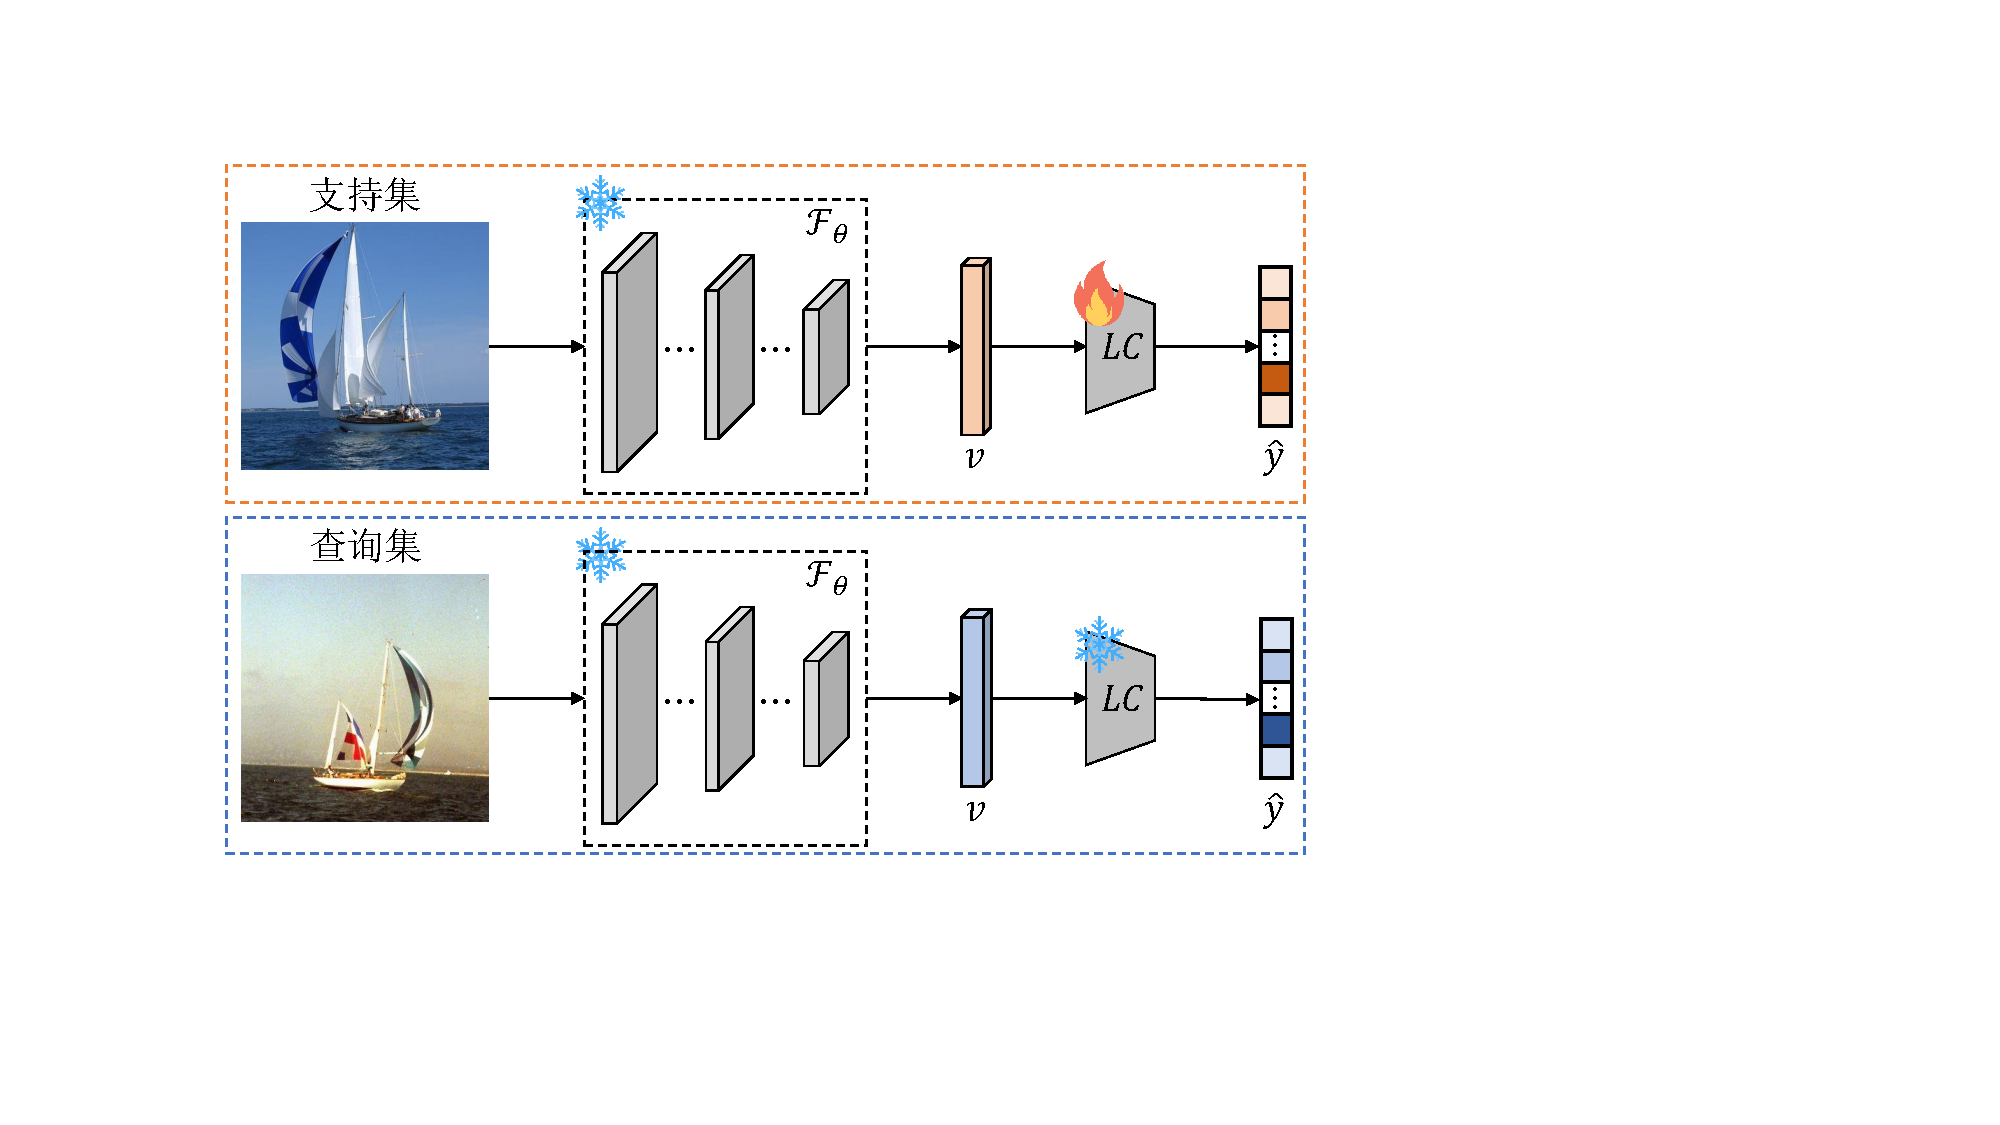
\includegraphics[width=0.8\columnwidth]{figures/MGSRCL/推理过程.pdf}
% \captionsetup{justification=justified,singlelinecheck=false}
\bicaption[MGSRCL模型推理过程示意图]{MGSRCL模型推理过程示意图。推理过程中,使用冻结参数的特征提取网络$\mathcal{F}_{\theta}$提取支持集与查询集的图像特征。其中,支持集特征被用来训练一个逻辑回归分类器$LC$,查询集特征则是用来测试分类器性能。}[Illustration of MGSRCL model inference process]{Illustration of MGSRCL model inference process. During the inference process, the feature extraction network $\mathcal{F}_{\theta}$ with frozen parameters is used to extract image features from both support set and query set. Herein, the support set features are utilized to train a logistic regression classifier $LC$, while the query set features are used to assess the classifier's performance.}
\vspace{-10pt}
\label{figure3: 推理过程}
\end{figure}

\section[\hspace{-2pt}实验设置及结果分析]{{\heiti\zihao{-3} \hspace{-8pt}实验设置及结果分析}}\label{section3: 实验设置及结果分析}
在本节中
\section[\hspace{-2pt}本章小结]{{\heiti\zihao{-3} \hspace{-8pt}本章小结}}\label{section3: 本章小结}

本章

\chapter[\hspace{0pt}基于语义-视觉多空间关系建模的少样本分类研究]{{\heiti\zihao{3}\hspace{0pt}基于语义-视觉多空间关系建模的少样本分类研究}}\label{chapter4: 基于语义-视觉多空间关系建模的少样本分类研究}
\removelofgap
\removelotgap

上一章研究了基于多粒度样本关系建模的少样本特征学习算法,通过充分挖掘不同粒度的样本关系提高了网络所提取特征的质量。然而,该算法仅在视觉空间对多种样本关系进行了建模,忽略了数据集中所隐含的丰富语义信息,限制了模型通过基类数据进行训练来学习新类数据知识的能力。因此,在上一章的基础上,本章主要研究基于语义-视觉多空间关系建模的少样本特征适配算法,通过引入语义信息并与视觉信息进行建模从而丰富模型所获得的信息,增强模型的泛化能力。本章内容共分为四节,\hyperref[section4: 引言]{第一节}介绍研究动机和方法概述;\hyperref[section4: 基于语义-视觉多空间关系建模的少样本特征适配算法]{第二节}介绍本章提出的基于语义-视觉多空间关系建模的少样本特征适配算法;\hyperref[section4: 实验设置及结果分析]{第三节}给出实验设置和结果分析;\hyperref[section4: 本章小结]{第四节}对本章进行小结。

\section[\hspace{-2pt}引言]{{\heiti\zihao{-3} \hspace{-8pt}引言}}\label{section4: 引言}

\section[\hspace{-2pt}基于语义-视觉多空间关系建模的少样本特征适配算法]{{\heiti\zihao{-3} \hspace{-8pt}基于语义-视觉多空间关系建模的少样本特征适配算法}}\label{section4: 基于语义-视觉多空间关系建模的少样本特征适配算法}

\section[\hspace{-2pt}实验设置及结果分析]{{\heiti\zihao{-3} \hspace{-8pt}实验设置及结果分析}}\label{section4: 实验设置及结果分析}

\section[\hspace{-2pt}本章小结]{{\heiti\zihao{-3} \hspace{-8pt}本章小结}}\label{section4: 本章小结}

本章研究基于语义-视觉多空间关系建模的少样本特征适配算法,针对少样本分类中仅根据少量视觉特征无法捕获类别代表性特征的缺点,引入语义信息作为视觉信息的补充,通过对语义-视觉多空间关系进行建模,提出了语义-视觉多空间映射适配模型(Semantic-Visual Multi-Space Mapping Adapter,简称SVMSMA),以丰富样本特征的信息来源,利用语义特征对视觉特征进行补充与修正,从而提升模型在新类上的泛化能力。SVMSMA模型使用单/多模态映射网络将样本语义特征映射到视觉空间获得单/多模态映射特征,并通过跨模态分类(CMC)模块与跨模态特征对齐(CMFA)模块对映射网络进行优化,以使得语义特征与视觉特征建立联系。测试过程中,本章方法将支持集的视觉特征、单模态映射特征、以及多模态映射特征共同作为分类器的训练数据,达到了较仅使用单一特征时更好的分类结果。在miniImageNet、tieredImageNet、CIFAR-FS和CUB-200-2011数据集的大量实验表明了SVMSMA方法的有效性。

综上所述,本章提出的基于语义-视觉多空间关系建模的少样本特征适配算法通过对语义-视觉多空间关系进行建模,充分利用语义信息对视觉信息进行了补充,丰富了样本特征信息来源,提升了模型的泛化能力。

\chapter[\hspace{0pt}模型评价与推广]{{\heiti\zihao{3}\hspace{0pt}模型评价与推广}}\label{chapter4: 模型评价与推广}
\removelofgap
\removelotgap

\section[\hspace{-2pt}主要结论]{{\heiti\zihao{-3} \hspace{-8pt}主要结论}}\label{section5: 主要结论}

本文针对LED显示器颜色转换与校正问题,建立了基于CIE Lab色彩空间和感知色差理论的数学模型,采用多种优化算法实现了高精度的颜色处理。主要研究结论如下:

\noindent\textbf{(1)BT.2020到sRGB颜色空间转换模型}

构建了基于$\Delta E_{00}$感知误差最小化的优化模型,通过差分进化算法求解最优线性映射矩阵。在50次独立实验中,平均$\Delta E_{00}$损失值为0.0744,远低于人眼可察觉阈值;色域面积差异控制在0.001以内,映射后色度三角与标准sRGB色域几乎完全重合。

\noindent\textbf{(2)多通道颜色空间转换神经网络模型}

设计了ColorNet神经网络架构,采用混合损失函数成功解决4通道到5通道的颜色转换问题。混合损失函数结合MSE数值精度与$\Delta E_{2000}$感知准确性,优先保证视觉效果;验证集上$\Delta E_{2000}$误差主要集中在较低范围。

\noindent\textbf{(3)LED显示器颜色校正优化模型}

建立了结合伽马校正与线性矩阵变换的综合校正模型,采用差分进化与L-BFGS-B混合优化策略。三种基色图像平均改善幅度达95.6\%,校正后平均色差降至0.095;100\%像素达到$\Delta E<1.0$的优秀标准;校正矩阵行列式值约0.10,保证了数值稳定性。

\section[\hspace{-2pt}模型优点]{{\heiti\zihao{-3} \hspace{-8pt}模型优点}}\label{section5: 模型优点}

\noindent\textbf{(1)理论基础扎实}:基于CIE Lab色彩空间和国际标准色差公式,确保了颜色处理的科学性和准确性。

\noindent\textbf{(2)技术方法先进}:采用差分进化算法、神经网络和混合优化策略,有效处理非线性、维度不匹配等复杂问题。

\noindent\textbf{(3)实用价值突出}:校正流程简洁高效,数值稳定性良好,实验验证充分,适合实际工程应用。

\section[\hspace{-2pt}不足与改进方向]{{\heiti\zihao{-3} \hspace{-8pt}不足与改进方向}}\label{section5: 不足与改进方向}

\noindent\textbf{(1)主要局限}

线性映射矩阵可能无法充分捕捉复杂的非线性颜色响应关系;神经网络模型使用模拟数据训练,与真实设备数据可能存在差异;对环境光照、设备老化等外在因素考虑有限。

\noindent\textbf{(2)改进方向}

探索非线性映射方法,结合多模态数据融合,开发实时自适应校正算法;将模型应用于HDR显示、VR/AR设备等专业领域;推动建立跨平台颜色校正标准,促进技术普及应用。

总之,本文为LED显示器颜色处理提供了完整的理论框架和实用解决方案,在颜色空间转换、多通道映射和颜色校正等关键环节均实现了技术突破,为高质量显示技术发展奠定了基础。

%\include{contents/yourFreeChoise}

\backmatter %%% 后置部分(致谢、参考文献、附录等)

%% 参考文献
% 顺序编码制:cqunumerical		
% 注意:至少需要引用一篇参考文献,否则下面两行会引起编译错误。
% \bibliographystyle{cqunumerical}
\bibliographystyle{gbt7714-numerical_new}
\bibliography{ref/refs}


%% 附录(按ABC...分节,证明、推导、程序、个人简历等)
\appendix
\chapter[附\hskip\ccwd{}\hskip\ccwd{}录]{{\heiti\zihao{3}附\hskip\ccwd{}\hskip\ccwd{}录}}

\section[\hspace{-2pt}作者在攻读硕士学位期间的论文目录]{{\heiti\zihao{-3} \hspace{-8pt}作者在攻读硕士学位期间的论文目录}}

%下面是盲审标记\cs{secretize}的用法,记得去\textsf{main.tex}开启盲审开关看效果:

% \circled{1}已发表论文

% \begin{enumerate}
%     \item \textbf{\secretize{XU X}}, \secretize{LIU K}, DAI P, et al. Joint task offloading and resource optimization in NOMA-based vehicular edge computing: A game-theoretic DRL approach[J]. Journal of Systems Architecture, 2023, 134: 102780. 影响因子: 5.836(2021), 4.497(5年) (中科院SCI 2区,对应本文第三章)
% 	\item \textbf{\secretize{许新操}}, \secretize{刘凯}, 刘春晖, 等. 基于势博弈的车载边缘计算信道分配方法[J]. 电子学报, 2021,49(5): 851-860. (EI 索引,CCF T1类中文高质量科技期刊,对应本文第三章)
% 	\item \textbf{ \secretize{XU X}}, \secretize{LIU K}, XIAO K, et al. Vehicular fog computing enabled real-time collision warning via trajectory calibration[J]. Mobile Networks and Applications, 2020, 25(6): 2482-2494. 影响因子: 3.077(2021), 2.92(5年) (中科院SCI 3区,对应本文第五章)
% \end{enumerate}
{
\small
\setlength{\baselineskip}{20pt}
\begin{enumerate}[label={[\arabic*]}, leftmargin=*]
\item \secretize{\textbf{Yin G}}, \secretize{Huang S}, He T, et al. Mirrored EAST: An Efficient Detector for Automatic Vehicle Identification Number Detection in the Wild[J]. IEEE Transactions on Industrial Informatics, 2023. (中科院SCI一区)
\item \secretize{\textbf{Yin G}}, Wang Y, Zhang Y, et al. Adversarial Bidirectional Feature Generation for Generalized Zero-Shot Learning Under Unreliable Semantics[C]//Chinese Conference on Pattern Recognition and Computer Vision (PRCV). Cham: Springer Nature Switzerland, 2022: 639-654.(CCF-C)
\item \secretize{\textbf{Yin G}}, Huangfu L, \secretize{Huang S}, et al. Rethinking the Sample Relations for Few-Shot Classification[J]. Image and Vision Computing. (中科院SCI三区,返修中)
\end{enumerate}
}


\section[\hspace{-2pt}作者在攻读硕士学位期间参与的科研项目]{{\heiti\zihao{-3} \hspace{-8pt}作者在攻读硕士学位期间参与的科研项目}}

{
\small
\setlength{\baselineskip}{20pt}
\begin{enumerate}[label={[\arabic*]}, leftmargin=*]
\item 国家自然科学基金面上项目,少样本学习特征生成与鲁棒性关键技术研究
% (No. 62176030)
\item 重庆市自然科学基金面上项目,文本描述协同的双向生成式少样本学习研究
\end{enumerate}
}

\newpage
\section[\hspace{-2pt}学位论文数据集]{{\heiti\zihao{-3} \hspace{-8pt}学位论文数据集}}

\begin{table}[h]
% \resizebox{\textwidth}{!}{%
\begin{tabular}{|cccccccccccc|}
\hline
\multicolumn{4}{|c|}{\heiti{关键词}}             & \multicolumn{4}{c|}{\heiti{密级}}   & \multicolumn{4}{c|}{\heiti{中图分类号}}                                    \\ \hline
\multicolumn{4}{|c|}{\begin{tabular}{c} 少样本分类; 关系建模; \\ 对比学习; 语义信息表示 \end{tabular}} & \multicolumn{4}{c|}{公开} & \multicolumn{4}{c|}{TP} \\ \hline
\multicolumn{3}{|c|}{\heiti{学位授予单位名称}} & \multicolumn{3}{c|}{\heiti{学位授予单位代码}}    & \multicolumn{3}{c|}{\heiti{学位类别}}  & \multicolumn{3}{c|}{\heiti{学位级别}}        \\ \hline
\multicolumn{3}{|c|}{\secretize{重庆大学}}     & \multicolumn{3}{c|}{\secretize{10611}}       & \multicolumn{3}{c|}{学术学位}  & \multicolumn{3}{c|}{硕士}          \\ \hline
\multicolumn{4}{|c|}{\heiti{论文题名}}            & \multicolumn{4}{c|}{\heiti{并列题名}} & \multicolumn{4}{c|}{\heiti{论文语种}}                                     \\ \hline
\multicolumn{4}{|c|}{\begin{tabular}{c}基于多元关系建模的少样\\本分类算法研究\end{tabular}}               & \multicolumn{4}{c|}{/}   & \multicolumn{4}{c|}{汉语} \\ \hline
\multicolumn{3}{|c|}{\heiti{作者姓名}}     & \multicolumn{3}{c|}{\secretize{尹国伟}}         & \multicolumn{3}{c|}{\heiti{学号}}    & \multicolumn{3}{c|}{\secretize{202124021028t}} \\ \hline
\multicolumn{6}{|c|}{\heiti{培养单位名称}}                                      & \multicolumn{6}{c|}{\heiti{培养单位代码}}                                   \\ \hline
\multicolumn{6}{|c|}{\secretize{重庆大学}}                                        & \multicolumn{6}{c|}{\secretize{10611}}                                    \\ \hline
\multicolumn{3}{|c|}{\heiti{学科专业}}     & \multicolumn{3}{c|}{\heiti{研究方向}}        & \multicolumn{3}{c|}{\heiti{学制}}    & \multicolumn{3}{c|}{\heiti{学位授予年}}       \\ \hline
\multicolumn{3}{|c|}{软件工程} & \multicolumn{3}{c|}{计算机视觉}         & \multicolumn{3}{c|}{3年}     & \multicolumn{3}{c|}{\secretize{2024年}}        \\ \hline
\multicolumn{3}{|c|}{\heiti{论文提交日期}}   & \multicolumn{3}{c|}{\secretize{2024年6月}}     & \multicolumn{3}{c|}{\heiti{论文总页数}} & \multicolumn{3}{c|}{\pageref{LastPage}}         \\ \hline
\multicolumn{3}{|c|}{\heiti{导师姓名}}     & \multicolumn{3}{c|}{\secretize{黄晟}}          & \multicolumn{3}{c|}{\heiti{职称}}    & \multicolumn{3}{c|}{教授}          \\ \hline
\multicolumn{6}{|c|}{\heiti{答辩委员会主席}}                                     & \multicolumn{6}{c|}{A}                                      \\ \hline
\multicolumn{12}{|c|}{\heiti{\begin{tabular}{c} 电子版论文提交格式\\ 文本(\checkmark) 图像() 视频()音频()多媒体()其他()\end{tabular}}}                              \\ \hline
\end{tabular}%
% }
\end{table}




%% 致谢
%\chapter[致\hskip\ccwd{}\hskip\ccwd{}谢]{{\heiti\zihao{3}致\hskip\ccwd{}\hskip\ccwd{}谢}}

% 这里用盲审环境包裹致谢,在开启盲审开关时,环境内部的内容不予渲染。
% \begin{secretizeEnv}

转眼间,从本科到硕士,已在重庆度过了七年,我的求学之路也告一段落。临近道别之际,借此机会给每一个支持和帮助过我的人们说一声感谢。

首先,感谢我的导师黄晟教授。在整个研究生阶段,导师给予了我无微不至的指导和关怀。是他的悉心教导,让我不断进步,最终完成了这篇毕业论文。在我遇到困难和挑战时,导师总是耐心倾听、指导并鼓励我,帮助我面对困难。在此,我向导师黄晟教授表示最诚挚的感谢!

同时,感谢重庆大学为我们提供了良好的学习环境和条件。学校的丰富资源和先进设施为我的研究提供了有力支持,让我能够顺利进行实验和调研。在这里,我结识了许多优秀的同学和朋友,他们的讨论和交流激发了我的灵感,也让我收获了很多。

另外,感谢我的家人。无论是在生活中还是在学业上,他们始终是我坚强的后盾,一直默默支持着我,使我能够安心学习。感谢我的女朋友魏欣钰女士,与我分享快乐,遇到挫折时给予我鼓励,帮助我渡过难关,不断前行。

感谢所有在论文写作过程中帮助过我的老师、同学和朋友们。尤其感谢张译、周锋涛、杨万里师兄入学以来的指导以及陈忠明、唐文浩、何涛同门提供的诸多帮助,是你们的建议、讨论和帮助让我不断改进论文,使其更加完善。在我即将踏上新征程之际,我会铭记你们的帮助和支持。

最后,感谢百忙之中参与评阅和答辩的各位专家、教授。

% \vfill
\vspace*{2em}
\begin{flushright}
{\CJKfontspec{STXingkai} \Large 尹国伟} \hspace*{3.5em}
\\  \hspace*{\fill} \\
{二〇二四年五月\hspace*{1em}于重庆}
\end{flushright}
% \end{secretizeEnv}

\end{document}